\chapter{Theoretical Framework} \label{ch2:theoframe}

In order to properly answer the established research questions an extensive review of the literature is needed. This chapter provides the fruits of that review. The knowledge provided here will guide the setup of the simulations, serve to inform the qualitative analyses of the discussion as well as form a reference for the suggestions for future research and work.

\section{Convexity}

The concept of convexity features heavily in the algorithms mentioned in this thesis. Thus, it is relevant to define its definition for the reader's convenience.

\begin{figure}[h]
	\centering
	\begin{minipage}[h]{0.2\textwidth}
		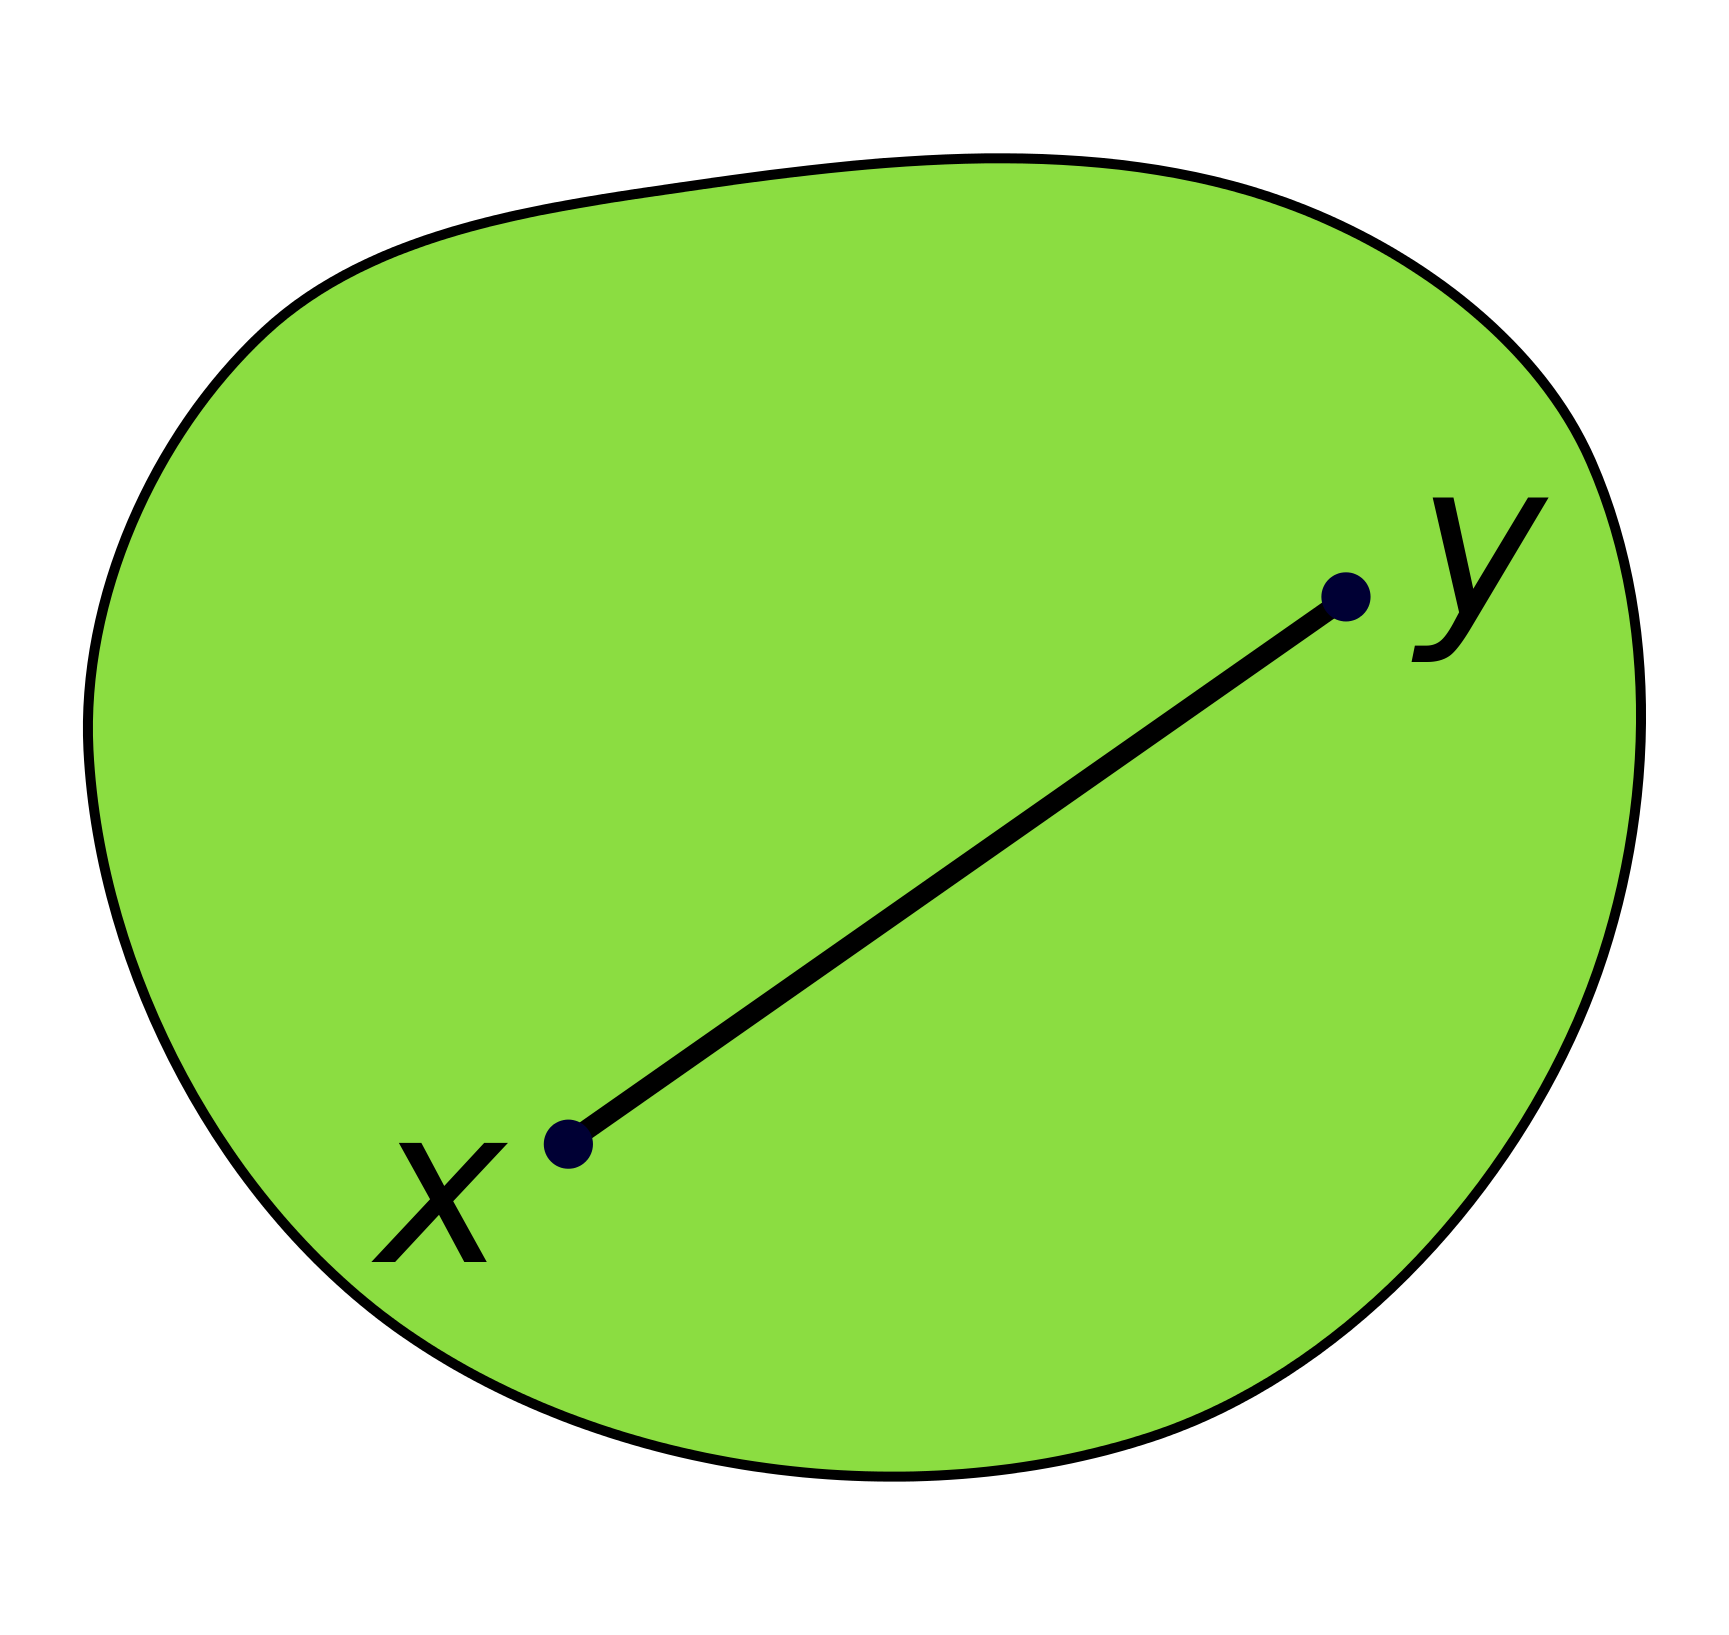
\includegraphics[width=1\textwidth]{import/ConvexPoly}
		\subcaption{A convex set. No matter what points x and y are chosen, the line between them will remain within the set.}
		\label{fig:ConvexPoly}
	\end{minipage}
	\hspace{1cm}
	\begin{minipage}[h]{0.2\textwidth}
		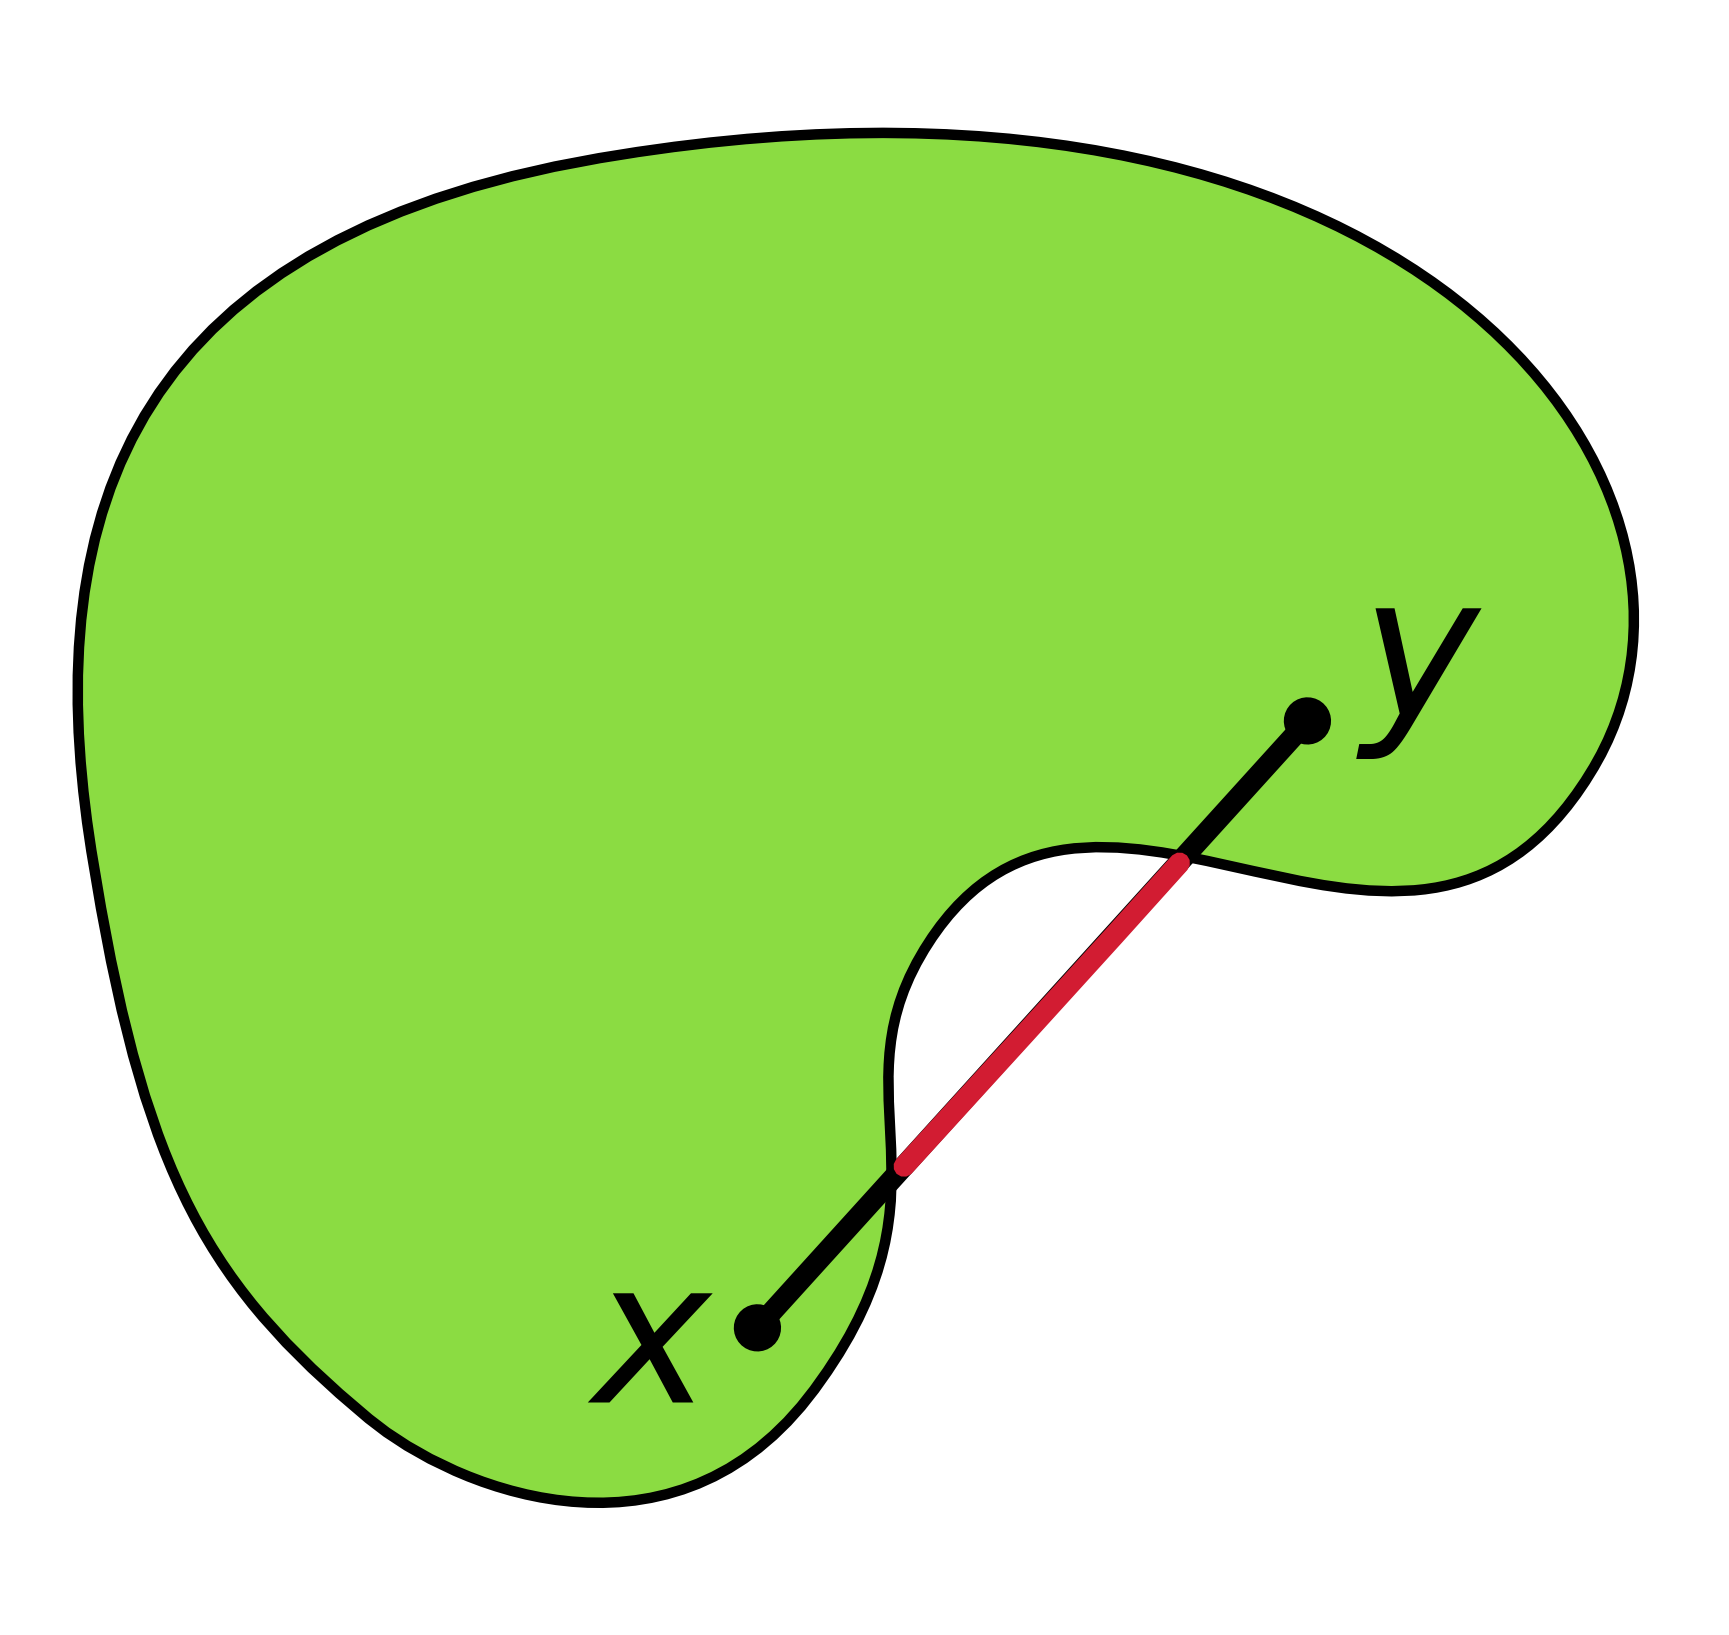
\includegraphics[width=1\textwidth]{import/ConcavePoly}
		\subcaption{A non-convex set. The red section signifies the part of the line not part of the set.}
		\label{fig:ConcavePoly}
	\end{minipage}
	\caption{\textbf{Source}: Images from Wikicommons released into the public domain.}
\end{figure}

A set is convex iff any line drawn between any arbitrary chosen pair of its points is fully contained within the set itself (see Figure \ref{fig:ConvexPoly}). If this criteria is not met, the set is non-convex (see Figure \ref{fig:ConcavePoly}). Similarly, a function is convex iff the epigraph (the set of points lying on or above its graph) is a convex set [\citeauthor{Sasane2016}] .

This can be expressed mathematically using the following inequality,
\begin{equation}
f(tx + (1 - t)y) \leq t f(x) + (1 - t)f(y), t \in (0, 1).
\end{equation}

Convex functions possess some properties that make them desirable in, among other fields, optimization. A problem consisting of finding the optimum of a function can be considered "well-posed" if the function as well as the feasible set (i.e., the set of values the variables are allowed to take) is convex [\citeauthor{Sasane2016}].

As an example, $x^2$ is a convex function possessing one global minimum at $x=0$. $x^3 + x^2$, on the contrary, is a non-convex function possessing a global minimum at $x=-\infty$, a global maximum at $x=\infty$, a local minimum at $x=0$ and a local maximum at $-\frac{2}{3}$. The existence of these local optima will cause problems for certain algorithms that rely on differentiating the function.


\section{Regarding Robotic Arms}

Robotic mechanisms are systems of rigid bodies connected by joints, whose positions and orientation are collectively termed the pose. One important topology is the one where the joints are connected in a serial chain, where each joint is connected to two others, except for the first and final link which are only connected to one other member [\citeauthor{Siciliano2016}].

A multitude of methods and formalisms have been developed to help in abstracting and representing the manipulator, as well as the environment in which it can actuate. One such formalism is that of configuration spaces. %comment away this paragraph if Kinematic Notation is added.

%A multitude of methods and formalisms have been developed that help in abstracting and representing the manipulator, as well as the environment in which it can move, two of which are presented here.

%\subsection{Kinematic Notation}
%
%One of the most famous kinematic notations is the \gls{DH} convention introduced in [\citeauthor{J.Dena}] in 1955, with variations building on it coming about later [\citeauthor{Siciliano2016}]. When using the \gls{DH} convention, coordinate frames, representing each \gls{DoF}, are attached at each joint such that there is one transformation for the joint $\mathcal{Z}$ and one for the link $\mathcal{X}$. Only four parameters, known as the \gls{DH} parameters, are necessary to define these transformations. These joint and link transformations are defined as follows,
%
%\begin{equation}
%\mathcal{Z}_i = \begin{bmatrix}
%	cos \theta_i & -sin \theta_i & 0 & 0 \\ sin \theta_i & cos \theta_i & 0 & 0 \\ 0 & 0 & 1 & d_i \\ 0 & 0 & 0 & 1
%\end{bmatrix}
%\label{DHZ} 
%\end{equation}
%\begin{equation}
%	\mathcal{X}_i = \begin{bmatrix}
%1 & 0 & 0 & r_{i} \\ 0 & cos \alpha_{i} & -sin \alpha_{i} & 0 \\ 0 & sin \alpha_{i} & cos \alpha_{i} & 0 \\ 0 & 0 & 0 & 1
%\end{bmatrix}, 
%\label{eq:DHX}
%\end{equation}
%such that 
%\begin{equation}
%\mathcal{T} = \mathcal{Z}_1\mathcal{X}_1, \dots, \mathcal{Z}_I\mathcal{X}_I
%\end{equation}
%describes a transformation from the base to the \gls{EE} of the robot.
%
%\begin{figure}[h]
%	\centering
%	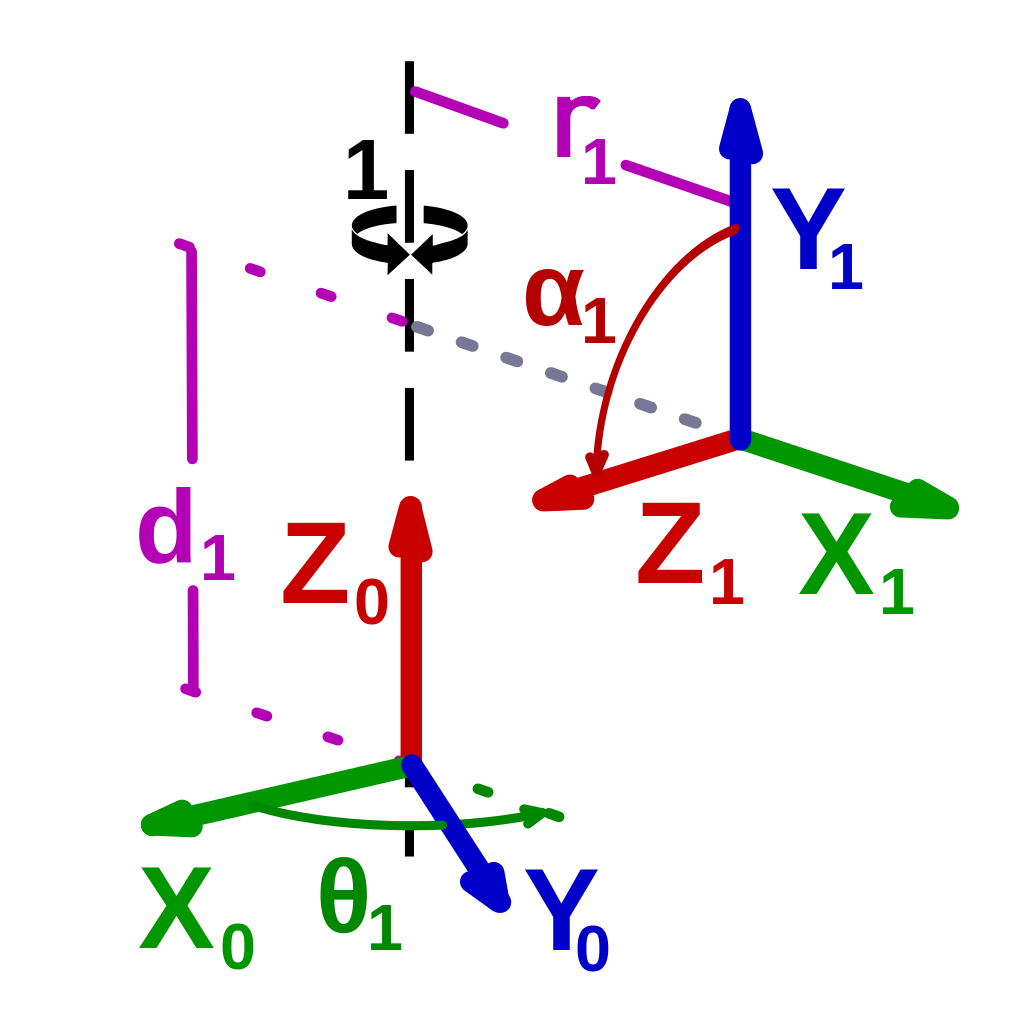
\includegraphics[width=0.45\textheight]{import/DH-illustration}
%	\caption{Two coordinate frames whose relationship are defined using the \gls{DH} convention. \textbf{Source}: Image originally from Wikicommons released into the public domain, with minor editing by this author.}%https://commons.wikimedia.org/wiki/File:Denavit-Hartenberg-Transformation.svg
%	\label{fig:DH}
%\end{figure}
%
%Note that a manipulator with $I$ joints will have $I+1$ links, due to each joint connecting each link. The joints go from 1 to $I$, and the links from 0 to $I$, with $i=0$ representing the base. Joint $i$ connects link $i-1$ to link $i$, and joint $i$ is considered fixed in respect to link $i-1$. Thus, when joint $i$ is actuated it is link $i$ that moves. Since there is no joint $i=0$, link $i=0$ is fixed [\citeauthor{Spong2004}]. One might see it as the unmoving link connecting joint $i=1$ to the the Earth.  
%
%The $\mathcal{Z}$ and $\mathcal{X}$ transformations can in turn be divided into a rotation and translation matrix each: $Rot(\theta)$ and $Trans(d)$ for $\mathcal{Z}$, and a $Rot(\alpha)$ and $Trans(r)$ for $\mathcal{X}$. The \gls{DH} parameters are defined as follows, defined for the current $i$ frame and illustrated in Figure \ref{fig:DH}:
%
%\begin{enumerate}
%	\item[$d_i$:] The \textit{Link Offset}. The distance between the $x_{i-1}$ axis and the $x_i$ axis, along the $z_{i-1}$ axis.        
%	\item[$\theta_i$:] The \textit{Joint Angle}. The angle around the $z_i$ axis between the $x_{i-1}$ axis and $x_i$ axis.
%	\item[$r_{i}$:] The \textit{Link Length}. The distance between the $z_{i-1}$ axis and the $z_i$ axis, along their common normal.
%	\item[$\alpha_{i}$:] The \textit{Link Twist}. The angle around the common normal between the $z_{i-1}$ and the $z_i$ axes.
%\end{enumerate}
%
%Because the \gls{DH} convention only relies on four parameters as opposed to six (as we are dealing with rotation and translation in 3D space) to define the relationships between the frames, issues with uniqueness can arise in specific cases [\citeauthor{Spong2004}]. Three cases are reviewed:
%
%\begin{enumerate}
%	\item[$\textbf{i}$] Coordinate axes $z_{i-1}$ and $z_i$ are not coplanar, in which case a unique line segment perpendicular (i.e., their common normal) to them connecting them exists. Axis $x_i$ is defined by this line, and the point where it intersects $z_i$ becomes the origin $O_i$. The vector defining the coordinate frames going between origins $O_{i-1}$ and $O_i$ is a linear combination of $x_i$ and $z_{i-1}$. This vector relates to the \gls{DH} parameters as follows: $d_i \cdot \hat{z}_{i-1} + r_i \cdot \hat{x}_i$, where the circumflex symbol denotes a unit vector. All the $DH$ parameters are uniquely defined.
%	
%	\item[$\textbf{ii}$] Coordinate axes $z_{i-1}$ and $z_i$ \textit{are} coplanar ($\alpha_i = 0$), in which case there is no uniquely defined normal. Axis $x_i$ is no longer specified completely, and one is free to slide $O_i$ anywhere along $z_i$. As a direct consequence $d_i$, which defines the translation of $O_i$ along the $z_i$ axis, can be arbitrarily chosen, but for simplicity it is convenient to set it as 0, thereby moving $O_i$ to the same "height" as $O_{i-1}$ along the coplanar z axes. The vector going between the origins can the be defined as $r_i \cdot \hat{x_i}$. 
%	
%	\item [$\textbf{iii}$] $z_i$ is not only parallel to $z_{i-1}$ but also intersects it. Not only is $\alpha_i = 0$, but so is $r_i$. $d_i$ is not defined as 0 as that would collapse $O_i$ into $O_{i-1}$ with only the angle $\theta_i$ between $x_i$ and $x_{i-1}$ as the difference. This case is useful when looking at certain \gls{EE} that are located on a straight link of $d_I$ length from the final joint.
% 
%\end{enumerate}
%
%Finally, in kinematics, there are two basic joints that yield 1 \gls{DoF}, namely \textit{revolute} joints and \textit{prismatic} joints. Revolute joints are joints which can rotate around an axis, i.e. when the joint is a rotary actuator. Prismatic joints are joints which translate, i.e. when the joint is a linear actuator. For revolute joints $d$ is fixed and $\theta$ varies, whereas for prismatic joints $\theta$ is fixed and $d$ varies. For both joint types $r$ and $\alpha$ are static, as the are associated with the link (i.e. $\mathcal{X}$) and not the joint ($\mathcal{Z}$) [\citeauthor{Spong2004}].

\subsection{Configuration Space} \label{subsec:cspace}
	
A useful way to abstract path planning problems is to transform them from the real space of reality into configuration space, or C-space [\citeauthor{Siciliano2016}]. C-space is the space containing all possible configurations of a manipulator, where each point single point in the C-space corresponds to a specific position and orientation [\citeauthor{Lozano-perez1983}]. 

The axes spanning the C-space each correspond to a \gls{DoF}, e.g. the angle of a revolute joint or the translation of a prismatic joint.  Thus, while the number of dimensions of the real space our robots work in is limited to $3$, the amount of dimensions of C-space is only limited by the number of DoF.

The big benefit of using C-space is that configurations resulting in collisions in real space due to the presence of objects will designate whole regions in it as forbidden. This will have consequences for some of the algorithms proposed here. 



\section{Algorithms That Plan} \label{sec:planalgo}

There is a fundamental need in robotics to have algorithms that work to transform high-level specifications of tasks set by humans (e.g. "grab that object"), into low-level instructions of how to move [\citeauthor{LaValle2006}]. The terms motion planning, trajectory planning, and so forth are often used to refer to these kinds of problems.

Motion planning has, since the late 1970s, been an active area of research. Initially the different approaches to the problem focused on complete planners, i.e. planners that return a solution provided that one exist, and return failure if not [\citeauthor{Karaman2010}]. It was however established that even the most simplistic motion planning problem, known as the piano mover's problem, is of complexity type PSPACE-hard (\textbf{P}olynomial \textbf{SPACE}). Thus, there is strong evidence that \textit{complete} planners are doomed to be computationally intractable, as the algorithm requires time growing exponentially with the number of DoF [\citeauthor{Reif1985}].

Algorithms which intend to be tractable thus approach the problem by relaxing the completeness requirement. Examples include [\citeauthor{Karaman2010}]:

\begin{enumerate}
	\item Resolution Completeness: A solution can be found if one exist provided that the resolution parameter of the algorithm is fine enough. Motion planning methods that are based on gridding or cell decomposition tend to fall into this category.
	\item Probabilistic Completeness: The probability of finding a solution, provided that one exists, approaches $1$ as the number of samples approaches infinity. Sampling-based algorithms fall under this.
\end{enumerate}



\subsection{A*} \label{subsec:Astar}

The A* (pronounced A \textit{star}) algorithm was first proposed in its seminal 1968 paper [\citeauthor{PeterE.HAR}]. It was developed as a solution to the problem of optimal graph traversal, i.e. that of finding the minimum cost path in a graph. Real life manifestations of that problem included optimal routing of telephone traffic, optimal maze navigation, and layout planning of printed circuit boards. The authors recognized that those problems were often approached in one of two ways: mathematically and heuristically. 

The mathematical approach typically dealt with properties of graphs as abstract mathematical objects, whose nodes would be orderly examined using algorithms that were mathematically proven to find the optimal solution. This approach, however, was not necessarily concerned with the \textit{computational feasibility} of the algorithms as much as with the guarantee of the optimal solution being found.

The heuristic approach makes use of domain-specific knowledge of the problem being represented with a graph in order to facilitate the search. For example, an AI strategy board game opponent can make use of expert knowledge to better evaluate the utility of specific states. A public transportation trip planner can make use of Euclidean distance and geographic information to avoid going through branches of the graph that will have the user be transported away from their goal. In contrast with the previously mentioned approach, this approach is typically not concerned with finding a \textit{minimum cost} solution as it is with finding \textit{a} solution, as fast as possible.

A* came about as an attempt by the authors of [\citeauthor{PeterE.HAR}] to combine these two approaches.

\subsubsection*{Regarding Graphs and Traversal}

A graph $G$ is composed of a set of $\{n_i\}$ nodes and $\{e_{ij}\}$ arcs between those nodes. If $e_{pq} \in \{e_{ij}\}$ then there is an arc between $n_p$ to $n_q$, and $n_q$ is in such a case a successor of $n_p$. Traversing that arc incurs a cost $c_{pq}$, which is a member of the overall set ${c_{ij}}$. Note that in many cases $c_{ij} \neq c_{ji}$ is possible, assuming that both arcs exist.

\begin{figure}
	\centering
	
\usetikzlibrary{shapes,fit}
\begin{tikzpicture}%[node distance = 3cm, auto,scale=0.85, every node/.style={scale=0.85}]
% Place nodes
\centering

\begin{scope}[every node/.style={circle,thick,draw}]
\node [shape=circle, draw=black] (A) at (0,0) {A};
\node [shape=circle, draw=black] (B) at (2,2) {B};
\node [shape=circle, draw=black] (C) at (2,-2) {C};
\end{scope}
% Draw edges
%\path [line] (BG) -- (RQ);
\path [line] (A) -- (B);
\path [line] (A) -- (C);
\path [line] (B) -- (C);
\begin{scope}[>={Stealth[black]},
	every node/.style={fill=white,circle},
	every edge/.style={draw=red,very thick}]
\path [->] (A) edge node {$1$} (B);
\path [->] (A) edge node {$5$} (C);
\path [->] (B) edge node {$3$} (C);

%\path [->] (B) edge[bend right=60] node {$1$} (E); 
\end{scope}



%\path [line] (SQ.east) --([shift={(5mm,0mm)}]SQ.east)--node[anchor=south] {} ([shift={(5mm,0mm)}]gather.east) -- (gather.east);

\end{tikzpicture}


	\caption{Three nodes $n_A$, $n_B$ and $n_C$ in a graph and the costs of traversing their arcs.}
	\label{fig:path_ex}
\end{figure}

Pairs of nodes do in general have multiple subsets of arcs connecting them. These are called paths. Figure \ref{fig:path_ex} illustrates a case where there are two paths between nodes $n_A$ and $n_C$, one of which is composed of one arc ($e_{AC}$) and the second of two arcs ($e_{AB}, e_{BC}$). Note also that the path composed of two arcs is of a lower total cost than the path composed of one.


An admissible algorithm could work as follows:

\begin{enumerate}
	\item Start from a start node $n_{s}$ and expand the node.
	\item List all the $K$ nodes $n_{1}, ..., n_{K}$  which are connected to $n_{s}$ by the edges $e_{s1}, ..., e_{sK}$, each of which are associated with a cost $c_{sk}$ for $k \in 1, ..., K$.
	\item Sort the nodes along their respective cost.
	\item Pick the node whose path has the lowest cost and check if it is the goal node. \begin{enumerate}
		\item If true, terminate and return path.
		\item If false, check if a cheaper path to the node exists in the memory bank.
		\begin{enumerate}
			\item If true, move on to the second cheapest node.
			\item If false, save to the memory bank as the cheapest path and expand the node.
		\end{enumerate}
	\end{enumerate}
	\item Sort all of the nodes according to costs of their paths. Duplicate nodes, representing new paths to the same nodes, can emerge.
	\item Repeat from Step 4.
\end{enumerate}
 
A memory bank from which to filter out already traversed paths is needed. Otherwise, using the graph in Figure \ref{fig:admis_ex} as an example, the algorithm could get stuck in a loop: $n_A \rightarrow n_B \rightarrow n_A \rightarrow n_B \rightarrow ...$. This algorithm would eventually return an optimal solution, but it would not necessarily do it fast enough, depending on the application and graph size.

%\begin{figure}[h]
%	\begin{subfigure}{.1\textwidth}
%		
\usetikzlibrary{shapes,fit}
\begin{tikzpicture}%[node distance = 3cm, auto,scale=0.85, every node/.style={scale=0.85}]
% Place nodes
\centering

\begin{scope}[every node/.style={circle,thick,draw}]
\node [shape=circle, draw=black] (A) at (0,0) {A};
\node [shape=circle, draw=black] (B) at (5,2) {B};
\node [shape=circle, draw=black] (C) at (5,0) {C};
\node [shape=circle, draw=black] (D) at (5,-2) {D};
\node [shape=circle, draw=black] (E) at (9, 3) {E};
\node [shape=circle, draw=black] (F) at (9, 1) {F};
\node [shape=circle, draw=black] (G) at (9, -1) {G};
\node [shape=circle, draw=black] (H) at (9, -3) {H};
\end{scope}

% Draw edges
%\path [line] (BG) -- (RQ);
%\path [line] (A) -- (B);
%\path [line] (A) -- (C);
%\path [line] (B) -- (C);
\begin{scope}[>={Stealth[black]},
	every node/.style={fill=white,circle},
	every edge/.style={draw=red,very thick}]
\path [->] (A) edge node {$1$} (B);
\path [->] (A) edge node {$9$} (C);
\path [->] (B) edge node {$3$} (C);
\path [->] (A) edge node {$5$} (D);
\path [->] (B) edge[bend right=60] node {$1$} (A);
\path [->] (E) edge[bend right=80] node {$6$} (A);
\path [->] (C) edge node {$8$} (D);
\path [->] (D) edge node {$5$} (H);
\path [->] (C) edge node {$4$} (F);
\path [->] (C) edge node {$5$} (H);
\path [->] (B) edge node {$2$} (E);
\path [->] (B) edge node {$10$} (F);
\path [->] (B) edge node {$13$} (H);
\path [->] (H) edge node {$2$} (G);
\path [->] (A) edge[bend right=40] node {$12$} (H);
\path [->] (E) edge[bend left=60] node {$1$} (H);
\path [->] (F) edge node {$4$} (G);
\path [->] (G) edge[bend right=45] node {$4$} (E);
\path [->] (E) edge[bend right=60] node {$3$} (B); 
\end{scope}



%\path [line] (SQ.east) --([shift={(5mm,0mm)}]SQ.east)--node[anchor=south] {} ([shift={(5mm,0mm)}]gather.east) -- (gather.east);

\end{tikzpicture}


%		\caption{A graph with arc costs.}
%		\label{fig:admis_ex}
%	\end{subfigure}
%	\newline
%	\begin{subfigure}{.1\textwidth}
%		\centering
%		
\usetikzlibrary{shapes,fit}
\begin{tikzpicture}%[node distance = 3cm, auto,scale=0.85, every node/.style={scale=0.85}]
% Place nodes
\centering

\begin{scope}[every node/.style={circle,thick,draw}]
\node [shape=circle, draw=black] (A) at (0,0) {A $9.1$};
\node [shape=circle, draw=black] (B) at (5,2) {B $4.1$};
\node [shape=circle, draw=black] (C) at (5,0) {C $4.1$};
\node [shape=circle, draw=black] (D) at (5,-2) {D $5.0$};
\node [shape=circle, draw=black] (E) at (9, 3) {E $2.0$};
\node [shape=circle, draw=black] (F) at (9, 1) {F $0.0$};
\node [shape=circle, draw=black] (G) at (9, -1) {G $2.0$};
\node [shape=circle, draw=black] (H) at (9, -3) {H $4.0$};
\end{scope}

% Draw edges
%\path [line] (BG) -- (RQ);
%\path [line] (A) -- (B);
%\path [line] (A) -- (C);
%\path [line] (B) -- (C);
\begin{scope}[>={Stealth[black]},
	every node/.style={fill=white,circle},
	every edge/.style={draw=red,very thick}]
\path [->] (A) edge (B);
\path [->] (A) edge (C);
\path [->] (B) edge (C);
\path [->] (A) edge (D);
\path [->] (B) edge[bend right=60] (A);
\path [->] (E) edge[bend right=80] (A);
\path [->] (C) edge (D);
\path [->] (D) edge (H);
\path [->] (C) edge (F);
\path [->] (C) edge (H);
\path [->] (B) edge (E);
\path [->] (B) edge (F);
\path [->] (B) edge (H);
\path [->] (H) edge (G);
\path [->] (A) edge[bend right=40] (H);
\path [->] (E) edge[bend left=60] (H);
\path [->] (F) edge (G);
\path [->] (G) edge[bend right=45] (E);
\path [->] (E) edge[bend right=60] (B); 
\end{scope}



%\path [line] (SQ.east) --([shift={(5mm,0mm)}]SQ.east)--node[anchor=south] {} ([shift={(5mm,0mm)}]gather.east) -- (gather.east);

\end{tikzpicture}


%		\caption{A variant on Figure \ref{fig:admis_ex} with Euclidean distance to goal node $n_F$ as a heuristic cost.}
%		\label{fig:heur_ex}
%	\end{subfigure}
%\caption{Two graphs.}
%\end{figure}

\begin{figure}[h]
		\centering
		
\usetikzlibrary{shapes,fit}
\begin{tikzpicture}%[node distance = 3cm, auto,scale=0.85, every node/.style={scale=0.85}]
% Place nodes
\centering

\begin{scope}[every node/.style={circle,thick,draw}]
\node [shape=circle, draw=black] (A) at (0,0) {A};
\node [shape=circle, draw=black] (B) at (5,2) {B};
\node [shape=circle, draw=black] (C) at (5,0) {C};
\node [shape=circle, draw=black] (D) at (5,-2) {D};
\node [shape=circle, draw=black] (E) at (9, 3) {E};
\node [shape=circle, draw=black] (F) at (9, 1) {F};
\node [shape=circle, draw=black] (G) at (9, -1) {G};
\node [shape=circle, draw=black] (H) at (9, -3) {H};
\end{scope}

% Draw edges
%\path [line] (BG) -- (RQ);
%\path [line] (A) -- (B);
%\path [line] (A) -- (C);
%\path [line] (B) -- (C);
\begin{scope}[>={Stealth[black]},
	every node/.style={fill=white,circle},
	every edge/.style={draw=red,very thick}]
\path [->] (A) edge node {$1$} (B);
\path [->] (A) edge node {$9$} (C);
\path [->] (B) edge node {$3$} (C);
\path [->] (A) edge node {$5$} (D);
\path [->] (B) edge[bend right=60] node {$1$} (A);
\path [->] (E) edge[bend right=80] node {$6$} (A);
\path [->] (C) edge node {$8$} (D);
\path [->] (D) edge node {$5$} (H);
\path [->] (C) edge node {$4$} (F);
\path [->] (C) edge node {$5$} (H);
\path [->] (B) edge node {$2$} (E);
\path [->] (B) edge node {$10$} (F);
\path [->] (B) edge node {$13$} (H);
\path [->] (H) edge node {$2$} (G);
\path [->] (A) edge[bend right=40] node {$12$} (H);
\path [->] (E) edge[bend left=60] node {$1$} (H);
\path [->] (F) edge node {$4$} (G);
\path [->] (G) edge[bend right=45] node {$4$} (E);
\path [->] (E) edge[bend right=60] node {$3$} (B); 
\end{scope}



%\path [line] (SQ.east) --([shift={(5mm,0mm)}]SQ.east)--node[anchor=south] {} ([shift={(5mm,0mm)}]gather.east) -- (gather.east);

\end{tikzpicture}


		\caption{A graph with arc costs.}
		\label{fig:admis_ex}
\end{figure}



Note the use of the verb expand in the algorithm. A different way of viewing a graph is to begin by only viewing the start node and disregarding the rest of the nodes. Then, the first level of nodes only emerge as a consequence of applying a successor operator $\Gamma$ to the starting node [\citeauthor{PeterE.HAR}]. In Figure \ref{fig:admis_ex}, if $n_A$ is set as the start node it would correspond to nodes $n_B$, $n_C$, $n_D$ and $n_H$.

In essence, the algorithm calculates the cost of the path to the node, which we can call $g(n)$, and attempts to minimize the cost of that all the way from the start node to the goal node.




%\begin{figure}
%	\centering
%	
\usetikzlibrary{shapes,fit}
\begin{tikzpicture}%[node distance = 3cm, auto,scale=0.85, every node/.style={scale=0.85}]
% Place nodes
\centering

\begin{scope}[every node/.style={circle,thick,draw}]
\node [shape=circle, draw=black] (A) at (0,0) {A};
\node [shape=circle, draw=black] (B) at (5,2) {B};
\node [shape=circle, draw=black] (C) at (5,0) {C};
\node [shape=circle, draw=black] (D) at (5,-2) {D};
\node [shape=circle, draw=black] (E) at (9, 3) {E};
\node [shape=circle, draw=black] (F) at (9, 1) {F};
\node [shape=circle, draw=black] (G) at (9, -1) {G};
\node [shape=circle, draw=black] (H) at (9, -3) {H};
\end{scope}

% Draw edges
%\path [line] (BG) -- (RQ);
%\path [line] (A) -- (B);
%\path [line] (A) -- (C);
%\path [line] (B) -- (C);
\begin{scope}[>={Stealth[black]},
	every node/.style={fill=white,circle},
	every edge/.style={draw=red,very thick}]
\path [->] (A) edge node {$1$} (B);
\path [->] (A) edge node {$9$} (C);
\path [->] (B) edge node {$3$} (C);
\path [->] (A) edge node {$5$} (D);
\path [->] (B) edge[bend right=60] node {$1$} (A);
\path [->] (E) edge[bend right=80] node {$6$} (A);
\path [->] (C) edge node {$8$} (D);
\path [->] (D) edge node {$5$} (H);
\path [->] (C) edge node {$4$} (F);
\path [->] (C) edge node {$5$} (H);
\path [->] (B) edge node {$2$} (E);
\path [->] (B) edge node {$10$} (F);
\path [->] (B) edge node {$13$} (H);
\path [->] (H) edge node {$2$} (G);
\path [->] (A) edge[bend right=40] node {$12$} (H);
\path [->] (E) edge[bend left=60] node {$1$} (H);
\path [->] (F) edge node {$4$} (G);
\path [->] (G) edge[bend right=45] node {$4$} (E);
\path [->] (E) edge[bend right=60] node {$3$} (B); 
\end{scope}



%\path [line] (SQ.east) --([shift={(5mm,0mm)}]SQ.east)--node[anchor=south] {} ([shift={(5mm,0mm)}]gather.east) -- (gather.east);

\end{tikzpicture}


%	\caption{A slightly more complicated graph than Figure \ref{fig:path_ex}.}
%	\label{fig:admis_ex}
%\end{figure}

\subsubsection*{Heuristics}

Instead of being concerned with the cost of traversing an arc to a node, one might instead want to assign a cost to the node in question that is independent of the path taken to reach it. The cost itself would be domain-specific, using a suitable heuristic. 

\begin{figure}[h]
	\centering
	
\usetikzlibrary{shapes,fit}
\begin{tikzpicture}%[node distance = 3cm, auto,scale=0.85, every node/.style={scale=0.85}]
% Place nodes
\centering

\begin{scope}[every node/.style={circle,thick,draw}]
\node [shape=circle, draw=black] (A) at (0,0) {A $9.1$};
\node [shape=circle, draw=black] (B) at (5,2) {B $4.1$};
\node [shape=circle, draw=black] (C) at (5,0) {C $4.1$};
\node [shape=circle, draw=black] (D) at (5,-2) {D $5.0$};
\node [shape=circle, draw=black] (E) at (9, 3) {E $2.0$};
\node [shape=circle, draw=black] (F) at (9, 1) {F $0.0$};
\node [shape=circle, draw=black] (G) at (9, -1) {G $2.0$};
\node [shape=circle, draw=black] (H) at (9, -3) {H $4.0$};
\end{scope}

% Draw edges
%\path [line] (BG) -- (RQ);
%\path [line] (A) -- (B);
%\path [line] (A) -- (C);
%\path [line] (B) -- (C);
\begin{scope}[>={Stealth[black]},
	every node/.style={fill=white,circle},
	every edge/.style={draw=red,very thick}]
\path [->] (A) edge (B);
\path [->] (A) edge (C);
\path [->] (B) edge (C);
\path [->] (A) edge (D);
\path [->] (B) edge[bend right=60] (A);
\path [->] (E) edge[bend right=80] (A);
\path [->] (C) edge (D);
\path [->] (D) edge (H);
\path [->] (C) edge (F);
\path [->] (C) edge (H);
\path [->] (B) edge (E);
\path [->] (B) edge (F);
\path [->] (B) edge (H);
\path [->] (H) edge (G);
\path [->] (A) edge[bend right=40] (H);
\path [->] (E) edge[bend left=60] (H);
\path [->] (F) edge (G);
\path [->] (G) edge[bend right=45] (E);
\path [->] (E) edge[bend right=60] (B); 
\end{scope}



%\path [line] (SQ.east) --([shift={(5mm,0mm)}]SQ.east)--node[anchor=south] {} ([shift={(5mm,0mm)}]gather.east) -- (gather.east);

\end{tikzpicture}


	\caption{A variant on Figure \ref{fig:admis_ex} with approximate Euclidean distance to goal node $n_F$ as a heuristic cost.}
	\label{fig:heur_ex}
\end{figure}


In navigation, the goal in is to minimize the distance between an object and the destination by moving the object to it. Thus, it makes intuitive sense to incorporate the distance as a heuristic cost, by for example calculating the Euclidean distance for each node to the goal node (i.e. the destination). Figure \ref{fig:heur_ex} gives an example of such a graph, where $n_F$ is the assigned goal node.

%\begin{figure}
%	\centering
%	
\usetikzlibrary{shapes,fit}
\begin{tikzpicture}%[node distance = 3cm, auto,scale=0.85, every node/.style={scale=0.85}]
% Place nodes
\centering

\begin{scope}[every node/.style={circle,thick,draw}]
\node [shape=circle, draw=black] (A) at (0,0) {A $9.1$};
\node [shape=circle, draw=black] (B) at (5,2) {B $4.1$};
\node [shape=circle, draw=black] (C) at (5,0) {C $4.1$};
\node [shape=circle, draw=black] (D) at (5,-2) {D $5.0$};
\node [shape=circle, draw=black] (E) at (9, 3) {E $2.0$};
\node [shape=circle, draw=black] (F) at (9, 1) {F $0.0$};
\node [shape=circle, draw=black] (G) at (9, -1) {G $2.0$};
\node [shape=circle, draw=black] (H) at (9, -3) {H $4.0$};
\end{scope}

% Draw edges
%\path [line] (BG) -- (RQ);
%\path [line] (A) -- (B);
%\path [line] (A) -- (C);
%\path [line] (B) -- (C);
\begin{scope}[>={Stealth[black]},
	every node/.style={fill=white,circle},
	every edge/.style={draw=red,very thick}]
\path [->] (A) edge (B);
\path [->] (A) edge (C);
\path [->] (B) edge (C);
\path [->] (A) edge (D);
\path [->] (B) edge[bend right=60] (A);
\path [->] (E) edge[bend right=80] (A);
\path [->] (C) edge (D);
\path [->] (D) edge (H);
\path [->] (C) edge (F);
\path [->] (C) edge (H);
\path [->] (B) edge (E);
\path [->] (B) edge (F);
\path [->] (B) edge (H);
\path [->] (H) edge (G);
\path [->] (A) edge[bend right=40] (H);
\path [->] (E) edge[bend left=60] (H);
\path [->] (F) edge (G);
\path [->] (G) edge[bend right=45] (E);
\path [->] (E) edge[bend right=60] (B); 
\end{scope}



%\path [line] (SQ.east) --([shift={(5mm,0mm)}]SQ.east)--node[anchor=south] {} ([shift={(5mm,0mm)}]gather.east) -- (gather.east);

\end{tikzpicture}


%	\caption{A variant on Figure \ref{fig:admis_ex} with Euclidean distance to goal node $n_F$ as a heuristic cost.}
%	\label{fig:heur_ex}
%\end{figure}



An algorithm making use of the Euclidean distance as the heuristic cost $h(n)$ to minimize in each step, in accordance with Figure \ref{fig:heur_ex}, with $n_A$ as the start node, would view $n_H$ as the cheapest node to expand on, regardless of the cost incurred to traverse to it. It would then expand on node $n_G$, then node $n_E$, before finally evaluating $n_B$ and then reach the goal $n_F$. 

As an algorithm working to make locally optimal decisions at every stage in the hope of reaching a globally optimal path, it can be considered a greedy algorithm [\citeauthor{Cormen2009}]. In this case however, while it would reach a solution in a reasonable amount of steps, it would not reach the globally optimal solution, which is in actuality $n_A \rightarrow n_B \rightarrow n_C \rightarrow n_F$.

\subsubsection*{Combining \textit{g(n)} and \textit{h(n)}}
A* works by combining the two cost functions, to produce the following
\begin{equation}
f(n) = g(n) + h(n),
\end{equation}
such that the cost evaluated when deciding the cheapest node takes into account both the path and heuristic costs. Thus, the strength of both approaches are combined.

Furthermore, in [\citeauthor{PeterE.HAR}], the authors prove that if the heuristics function chosen is \textit{admissible}, the algorithm is guaranteed to return a least-cost path from start to goal. An admissible heuristic is a heuristics function that does not over-estimate the actual cost to get to the goal.
\subsubsection*{A* in Motion Planning}

A* by itself is a path planning algorithm, in that it produces a plan for how to progress through many states before ending at a goal (provided that such a path exists). 

It is by combining it with the concept of the C-space mentioned in Section \ref{subsec:cspace} that motion planning is achieved, as the path produced by the algorithm corresponds to specific joint configurations of the robot. Feedback control policies can be used to have the joints actuate along the motion plan.

\begin{figure}[!h]
	\begin{minipage}[t]{4 cm}
		\usetikzlibrary{shapes,fit}
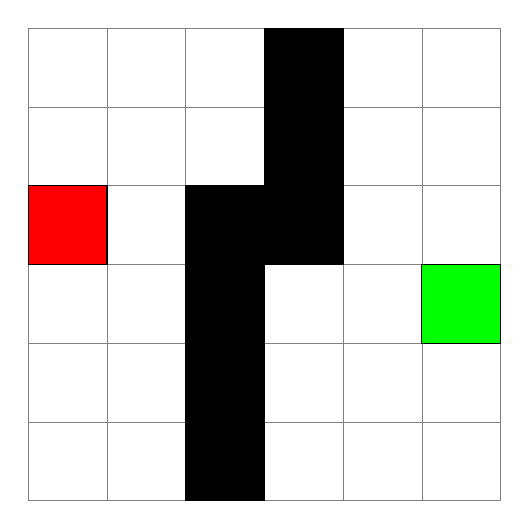
\begin{tikzpicture}%[node distance = 3cm, auto,scale=0.85, every node/.style={scale=0.85}]
% Place nodes
\centering

\draw[step=1cm,gray,very thin] (0,0) grid (6,6);

\filldraw[fill=red] (0,3) rectangle (1,4);

\filldraw[fill=green] (5,2) rectangle (6,3);

\filldraw[fill=black] (2,0) rectangle (3,4);
\filldraw[fill=black] (3,6) rectangle (4,3);

\end{tikzpicture}




	\end{minipage}
	\hspace{2.5cm}
	\begin{minipage}[t]{4 cm}
		\usetikzlibrary{shapes,fit}
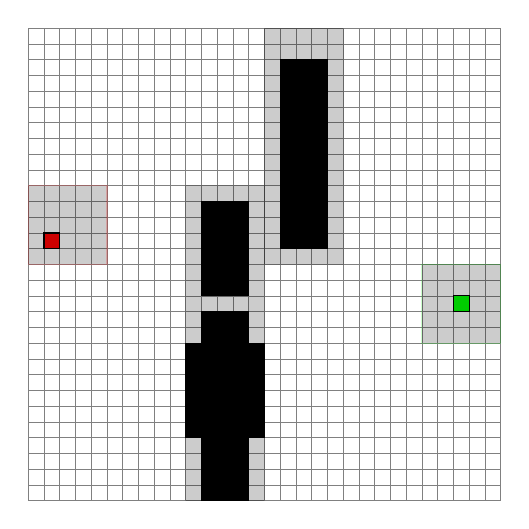
\begin{tikzpicture}%[node distance = 3cm, auto,scale=0.85, every node/.style={scale=0.85}]
% Place nodes
\centering

\draw[step=0.2cm,gray,very thin] (0,0) grid (6,6);

\filldraw[fill=red] (0.2, 3.2) rectangle (0.4, 3.4);

\filldraw[fill=green] (5.4, 2.4) rectangle (5.6,2.6);

\filldraw[fill=black] (2.2, 0) rectangle (2.8, 2.4); %bottom left
\filldraw[fill=black] (2, 0.8) rectangle (3, 2); %bottom left

\filldraw[fill=black] (2.2, 2.6) rectangle (2.8, 3.8 ); %upper left

\filldraw[fill=black] (3.2 , 5.6) rectangle (3.8, 3.2); %upper right



\filldraw[draw=red, opacity=0.2] (0,3) rectangle (1,4);

\filldraw[draw=green, opacity=0.2] (5,2) rectangle (6,3);

\filldraw[draw=black, opacity=0.2] (2,0) rectangle (3,4);
\filldraw[draw=black, opacity=0.2] (3,6) rectangle (4,3);


\end{tikzpicture}
	\end{minipage}
\caption{The same environment, represented with two grids of different resolutions, 1 cm and 0.2 cm step size respectively. Red represents the start state, green the goal state and black obstacles. The gray outline is used as a visual aid.} 
\label{fig:grids_reso_ex}
\end{figure}

%{\color{red} Red}, {\color{green} green

A* used in this way falls into the category of algorithms mentioned in Section \ref{subsec:cspace} as being resolution complete. Figure \ref{fig:grids_reso_ex} illustrates this concept. Both figures represent a grid representation of an environment in which a path from the red square to the green square must be found. In reality, a path does exist, but the algorithm's ability to find it is dependent on the grid resolution that has been set. Hence, no solution is available in the left case, but several exist in the right case. As the resolution goes to infinity, so does the computational challenge. 

In essence, an infinitely fine grid, with infinitely many nodes and arcs between them, would result in a complete but wholly intractable planner, as mentioned in Section \ref{sec:planalgo}. The exponential nature of the grid means that by increasing the resolution 5x (i.e., reducing the width of the squares by a factor 5), 25x more \textit{square} nodes emerge. In the 3D world, this would be a cubical increase, with 125x more cubic nodes replacing every 1 cube. 

Some methods have been developed to mitigate this problem, such as making the grid variable. Occupied grids could be recursively divided into finer grids, while free grids remain coarse. [\citeauthor{Kirby2009}] presented an algorithm designed to be used in real-time navigation path planning, where only the space close to the robot (which is of high relevance) is divided. Meanwhile, areas of the grid farther away are left coarse. Even then, while the computational strain is lessened, the issue of choosing the right resolution remains.

\subsection{Artificial Potential Fields} \label{subsec:APF}
A different planning algorithm, which draws inspiration from physics, is the \gls{APF} algorithm. In the \gls{APF} algorithm, a potential field is defined for the world. The manipulator moves in this field and experiences forces: repulsive forces are exerted from obstacles, and an attractive force is exerted from the goal point. 

The generalized kinetic energy equation for a holonomic articulated mechanism can be defined as follows,
\begin{equation}
	T(x, \dot{x}) = \frac{\dot{x}\Lambda(x)\dot{x}}{2}
\end{equation}
where $\Lambda(x)$ designates the symmetric matrix of the quadratic form, i.e. the kinetic energy matrix. Using the Lagrangian formalism, the equations defining the \gls{EE} motions are given by
\begin{equation}
	\frac{d}{dt}\left(\frac{\delta L}{\delta x}\right) - \frac{\delta L}{\delta x} = F,
\end{equation}
where the Lagrangian function is
\begin{equation} \label{eq:Lagr}
	L(x,\dot{x}) = T(x, \dot{x}) - U(x),
\end{equation}
and U(x) is defined as the potential energy of the gravity. F is the operational force vector. [\citeauthor{Khatib}] further develops and defines these equations in the form
\begin{equation}
	\Lambda(x)\ddot{x} + \mu(x, \dot{x}) + p(x) = F,
	\label{eq:Khatib4}
\end{equation}
with $\mu(x,\dot{x})$ as the centrifugal and Coriolis forces and $p(x)$ the forces of gravity.

%Controlling the manipulator is based using $F$ as a command vector, and in order to produce the command specific forces $\Gamma$ (different from the successor function mentioned in Section \ref{subsec:Astar}) need to be applied with joint-based actuators The relationship between $F$ and $\Gamma$ are given by the kinematics function
%\begin{equation}
%	\Gamma = J^T(q)F,
%\end{equation}
%where $q$ is the vector of dimension \textit{n} representing the joint coordinates, and $J(q)$) the Jacobian matrix relating joint angles to the \gls{EE} position. Equation \ref{eq:Khatib4} can be rewritten to
%\begin{equation}
%	F = \Lambda(x)F^* + \mu(x,\dot{x}) + p(x),
%\end{equation}
%were the vector $F^*$ has been added to represent the command vector a decoupled \gls{EE} which is equivalent to a single unit mass.

For the case of a single obstacle, the following equation can be set up,
\begin{equation}
	U_{art} = U_{x_d} + U_O 
\end{equation}
where $U_{O}$ refers to the field generated by the obstacle and $U_{x_d}$ by the goal at position $x_d$.  The $U(x)$ term in Equation \ref{eq:Lagr} can thus be redefined as
\begin{equation}
	U(x) = U_{art}(x) + U_g(x),
\end{equation}
as in addition to the gravitational field (represented by $U_g$), there is also the addition of the new artificial potential fields. Finally, we obtain the forces the end effector experiences by taking the negative of the gradient of these field functions:
\begin{equation}
	F^*_{art} = F*_{x_d} + F*_O = -\frac{\delta U_{x_d}}{\delta x} -\frac{\delta U_O}{\delta x}.
\end{equation}
The attractive potential field of the goal point is simply
\begin{equation}
	U_{x_d}(x) = \frac{k_p(x - x_d)^2}{2},
\end{equation}
where $k_p$ is a proportional control parameter affecting the strength of the attraction. $U_{O}(x)$ is a little more complicated to decide on, but it is selected such that the \gls{APF} $U_{art}(x)$ as a whole is a positive continuous and differentiable function which reaches a zero minimum when $x = x_d$. It should be designed such that it meets the manipulator's stability condition, creates a potential barrier at each point on the obstacle's surface (a barrier that becomes negligible beyond the surface) and is a non-negative continuous and differentiable function. [\citeauthor{Khatib}] coined the term FIRAS function, stemming from \textit{\textbf{F}orce \textbf{I}nducing an \textbf{A}rtificial \textbf{R}epulsion from the \textbf{S}urface} (but in French) for the force created by $U_O(x)$.

One example function proposed in [\citeauthor{Khatib1980}] is the following function:

\begin{equation}
U_O(x) = \begin{cases} 
	\frac{\eta \left(\frac{1}{\rho} - \frac{1}{\rho_0}\right)^2}{2} & \text{\textit{if}  } \rho \leq \rho_0 \\
	0 & \text{\textit{if}  } \rho > \rho_0 
\end{cases}
\label{eq:discPotF}
\end{equation}
where $\rho$ is the closest distance to the obstacle, $\rho_0$ a distance limit set by the user and $\eta$ a parameter adjusting the force strength. For distances above the distance limit the function is cut off.

\begin{figure}[h]
	\centering
	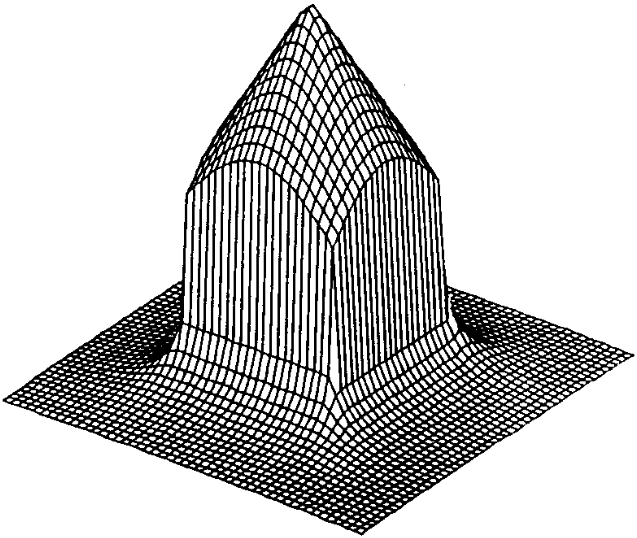
\includegraphics[width=0.5\textwidth]{import/APF_Obstacle.png}
	\caption{A potential field function. \textbf{Source}: [\citeauthor{Warren1989}].}
	\label{fig:APF_PotField}
\end{figure}

Figure \ref{fig:APF_PotField} shows how a discontinuous potential field might look like. For further in-depth information regarding the control theory, potential artificial potential functions and more, see [\citeauthor{Khatib}].

It is worth pointing out that \gls{SQ} have been used to model obstacles for \gls{APF}. \textit{Superquadric Potentials} are discussed in [\citeauthor{Volpe1990}], as their simple mathematical expression allow for creating \textit{deformable} (see Section \ref{subsubsec:SQDeform}) \gls{SQ}-based potential functions that can vary their shape as a function of distance.

[\citeauthor{Khatib}] used the \gls{APF} in real space, but others such as [\citeauthor{Warren1989}] and [\citeauthor{Volpe1990}] have used it to navigate in the C-space, providing an alternative to graph-searching algorithms like A*. By limiting to real space and avoiding the conversion to C-space, along with the fact that real space has only three dimensions, the algorithm solution time is reduced [\citeauthor{Warren1989}]. But the computational cost increases quickly as a function of the manipulator's \gls{DoF}, at the very least quadratically [\citeauthor{Volpe1990}], making them more suitable for offline planing than real-time obstacle avoidance with dynamic obstacles. Regardless, the \gls{APF} algorithm suffers from a fundamental problem of dealing with "local minima".

\subsubsection{The Local Minima Problem} \label{subsubsec:localminima}

\begin{figure}[!h]
	\begin{minipage}[t]{4 cm}
		
\pgfplotsset{width=7cm,compat=1.16}

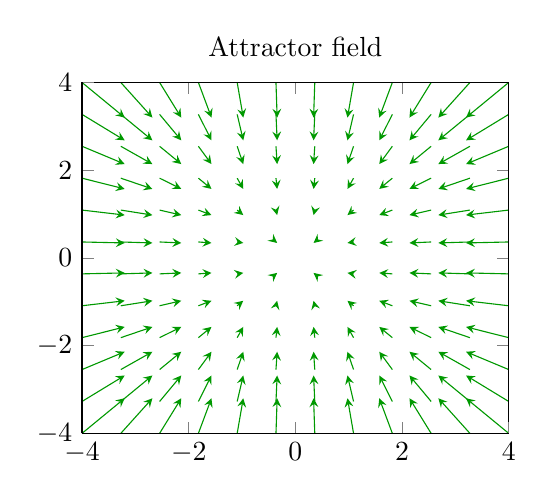
\begin{tikzpicture} 
	\begin{axis}[ 
		title={Attractor field}, 
		domain=-4:4, 
		view={0}{90}, 
		axis background/.style={fill=white}, 
	] 

		\addplot3[green!60!black, 
			quiver={ 
				u={-x*abs(x)^0.5}, 
				v={-y*abs(y)^0.5}, 
				scale arrows=0.1, 
			}, 
			-stealth,samples=12] 
				{0}; 
	\end{axis} 
\end{tikzpicture}
	\end{minipage}
	\hspace{2.5cm}
	\begin{minipage}[t]{4 cm}
		
\pgfplotsset{width=7cm,compat=1.16}

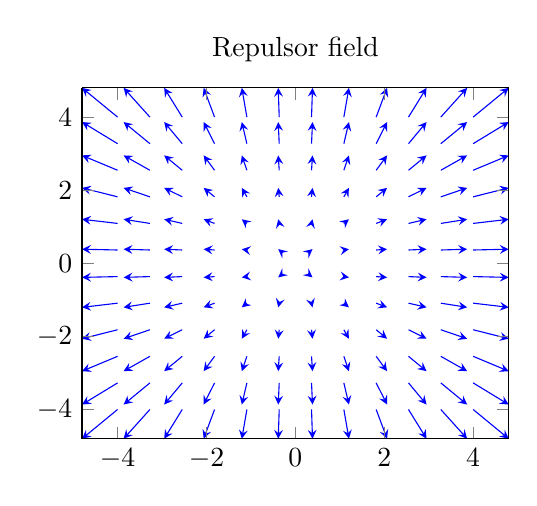
\begin{tikzpicture} 
	\begin{axis}[ 
		title={Repulsor field}, 
		domain=-4:4, 
		view={0}{90}, 
		axis background/.style={fill=white}, 
	] 

		\addplot3[blue, 
			quiver={ 
				u={x*abs(x)^0.5}, 
				v={y*abs(y)^0.5}, 
				scale arrows=0.1, 
			}, 
			-stealth,samples=12] 
				{0}; 
	\end{axis} 
\end{tikzpicture}
	\end{minipage}
	\caption{Two vector fields.} 
	\label{fig:apf_maxmin_ex}
\end{figure}

The fields in Figure \ref{fig:apf_maxmin_ex} could represent the forces guiding the \gls{EE} in space, with the goal point creating an attractor field from the point-of-view of the \gls{EE} and each obstacle creating a form of repulsive field. An unfortunate constellation of obstacle placements could result in certain points having prohibitively low values (depending on factors of thresholding, discretization, etc) following a summation of vectors. In other words, these points represent local minima which a \gls{EE}, mobile robot, etc could become trapped in ([\citeauthor{Lahouar2006}], [\citeauthor{Lindemann2005}], [\citeauthor{Tahir2018}]).

Note that functions describing these fields are continuous, but in reality discontinuous functions can be used (e.g., Equation \ref{eq:discPotF}). The $\rho_0$ variable means that the obstacle will only affect the overall $U_{art}$ within $\rho_0$ length units, which could mitigate the problem of local minimas. On the other hand, that distance must be properly set in relation to the maximum actuation speed. If $\rho_0$ is set to low the robot might not be able to decelerate itself in time to avoid impact.

\subsection{Model Predictive Control}

\gls{MPC} is slightly different from the other algorithms presented in that it belongs to the field of control, specifically optimal control.

Using an understanding of the internal dynamics of the plant model, a recorded history of the past control inputs $u$ and past measured outputs $y$, it iteratively explores state trajectories emanating from the current state at time $t$ (continuous) or $k$ (discrete). Then, it produces a cost-minimizing control strategy $u(\tau)$ (for $\tau \in [t, t + T]$) using a cost function $J$. Afterwards, it discards all the calculated future control moves but the next control move $u^+$ and implements it, before sampling the plant state again and repeating the process, sliding the time horizon forward ([\citeauthor{Hoy2012}], [\citeauthor{Wang2009a}]).

$J$ is designed to steer the control algorithm. One potential cost function, looking at a simple \gls{LQ} control example in the discrete domain (though \gls{MPC} is not limited to this problem statement) [\citeauthor{Rawlings2012}], could be the following,
\begin{equation}
J(x, u)=\frac{1}{2} \sum_{k=0}^{N-1}\left[x(k)'Qx(k) + u(k)'Ru(k)\right] + \frac{1}{2}x(N)'P_fx(N),
\label{eq:JMPCcost}
\end{equation}
subject to,
\begin{align}
x^+ = Ax + Bu, \\
y = Cx + Du.
\label{eq:discTimeLinearModel}
\end{align}
Due to the principle of receding horizon control where only current information of the plant is required for prediction and control, it is implicitly assumed that the input $u(k)$ cannot affect the output $y(k)$ at the same time. Thus, in MPC literature ([\citeauthor{Hoy2012}], [\citeauthor{Wang2009a}]) matrix $D$ is typically set as $D=0$. 

The cost functon in Equation \ref{eq:JMPCcost} measures the square deviation of the trajectory of $x(k)$ and $u(k)$ from zero, such that the algorithm will work to minimize them. Matrices $Q$ and $R$ have specific uses as tuning parameters [\citeauthor{Rawlings2012}]. 

Large values of $Q$ in comparison to $R$ means that the algorithm will penalize large deviations in state values, resulting in a more aggressive control. The reverse, large values of $R$ relative to $Q$, represents a wish to keep the magnitude of the control signals small, at the cost of slower convergence. Perhaps, due to concerns of energy consumption or wear and tear on the actuator, this is preferable. $P_f$ is there to specifically target the final state value (of the time horizon) for the sake of generality. 

In order to ensure the existence of a unique solution to the optimal control problem, matrices $Q$, $P_f$ and $R$ are \textit{real} and \textit{symmetric}; $Q$ and $P_f$ are \textit{positive semidefinite} ($\succeq 0$); and $R$ is \textit{positive definite} ($\succ 0$) ([\citeauthor{Rawlings2012}], [\citeauthor{Richter2012}]).

It is worth mentioning that under certain circumstances in linear \gls{MPC}, such as when the prediction horizon is large, the optimal control trajectory $u$ converges to that of an underlying optimal control trajectory given by a discrete-time \gls{LQ}-regulator with the same weight matrix $Q$ and $R$ [\citeauthor{Wang2009a}].

\subsubsection{Constraints}

The manipulated control inputs to various physical systems tend to be bounded, whether they be valve positions, voltages, torques and so forth [\citeauthor{Rawlings2012}]. It is possible to encode these hard limits using \gls{MPC}, in the following manner,
\begin{equation}
Eu(k) \leq e,
\end{equation}
in which,
\begin{equation}
E = \left[ \begin{array}{cc}
I\\ -I
\end{array} \right],
\hspace{1cm}
e = \left[\begin{array}{cc}
u^{max} \\-u^{min}
\end{array} \right],
\end{equation} 
are used to express simple bounds like,
\begin{equation}
u^{min} \leq u(k) \leq u^{max},
\end{equation}
where $u^{min}$ and $u^{max}$ represent the lower and upper bounds respectively, and $k$ is a non-negative integer. It is also possible to impose constraints on states or outputs. These can be stated analogously as,
\begin{equation}
Fx(k) \leq f.
\end{equation}
Limits on the control inputs $u$ are typically hard limits imposed by the physical system, whereas the constraints on the state output are typically imposed for reasons of safety, operability, product quality and such [\citeauthor{Rawlings2012}]. In other words, in the former case, if the controller does not respect the constraints then the physical system will naturally reinforce them. It is also possible to incorporate hard limits on the rate of change, by expanding the state variable with the previous control input value,
\begin{equation}
\tilde{x}(k) = \left[\begin{array}{cc}
x(k)\\ u(k-1)
\end{array}\right],
\end{equation}
creating an augmented system model,
\begin{align}
\tilde{x}^+ = \tilde{A}\tilde{x} + \tilde{B}u, \\
y = \tilde{C}\tilde{x} + Du,
\end{align}
where,
\begin{equation}
\tilde{A} = \left[ \begin{array}{cc}
A & 0\\ 0 & 0
\end{array} \right],
\hspace{1cm}
\tilde{B} = \left[\begin{array}{cc}
B \\ I
\end{array} \right],
\hspace{1cm}
\tilde{C} = \left[\begin{array}{cc}
C & 0
\end{array}\right].
\end{equation}
A constraint on the rate of change,
\begin{equation}
\Delta^{min} \leq u(k) - u(k-1) \leq \Delta^{max},
\end{equation}
is then formulated as,
\begin{equation}
	F\tilde{x}(k) + Eu(k)\leq e,
\end{equation}
where,
\begin{equation}
F = \left[ \begin{array}{cc}
0 & -I\\ 0 & I
\end{array} \right],
\hspace{1cm}
E = \left[\begin{array}{cc}
I \\ -I
\end{array} \right],
\hspace{1cm}
e = \left[\begin{array}{cc}
\Delta^{max} \\ -\Delta^{min}
\end{array}\right].
\end{equation}

Linear inequalities like these are useful when looking at linear systems, but the controller of the analysis is not significantly simplified by using them when looking at nonlinear systems [\citeauthor{Rawlings2012}]. Thus, we might as well generalize the constraints to memberships of sets:

\begin{equation}
x(k) \in \mathbb{X}, \hspace{1cm} u(k) \in \mathbb{U}, \hspace{1cm} k \in \mathbb{I}_{\geq 0},
\end{equation}

where $\mathbb{X}$ is the set of allowable states, $\mathbb{U}$ the set of allowable control inputs, and $\mathbb{I}_{\geq 0}$ the set of non-negative integers. 

Without constraints the model predictive control scheme devolves into a state feedback control system whose gain is chosen from minimizing a finite prediction horizon cost [\citeauthor{Wang2009a}]. Analytical and numerical results can be used to demonstrate the equivalence between the continuous-time \gls{MPC} and the classical \gls{LQ}-regulator for this case. 

This flexibility in being able to set the constraints is one of the benefits of using \gls{MPC}. If constraints are not set, it is of vital importance to come up with another way of handling control signal saturation, as it may severely deteriorate the performance. While feasible with \gls{SISO} systems, for \gls{MIMO} systems the limits of system operation appear in many forms (e.g, limits on each control signal, each control's systems respective $\Delta u(k)$, various state variables, etc). Working out the individual staturation limits in a co-ordinated manner becomes a very complex task, which motivates the use of \gls{MPC} and the constrained control framework that it brings.

\subsubsection{MPC for Guidance}\label{subsubsec:MPC4Guidance}

\gls{MPC} has received interest in vehicle navigation and steering. A strength of \gls{MPC} in active steering control is that it relies on a model predictive framework, which works to predict the outcome of the system. Due to this ability to project into the future, or "look-ahead", \gls{MPC} can be utilized to generate obstacle-avoiding trajectories [\citeauthor{Park2009}].

The authors of [\citeauthor{Marzat2017}] used \gls{MPC} to guide an autonomous \gls{MAV} to avoid obstacles in an cluttered indoor environment. The so-called \textit{Reactive} \gls{MPC} algorithm consists of having the \gls{MAV} follow a given reference trajectory defined in terms of positions $\xi(k)^r$ and velocities $V(k)^r$. This can be used regardless if a whole trajectory has been specified previously, or if only the goal point has been set. In the former case, interpolation is done in order to fit the discretization with the \gls{MPC} time step, and in the latter case the sequence is built with a constant nominal velocity $v_{nom}$ and the \gls{MPC} time step (with velocity ramps at the beginning and at the end).

At each time step, when producing the control scheme and emanating state trajectory, the algorithm checks if it \gls{MAV} will collide with an obstacle (or enter within a safety margin to it) and will add a corrective component to the control input that will cause it to deviate from the plan. The authors defined the following equation,

\begin{equation}
u(k) = u(k)^n + \textbf{1}^{obs}_k u(k)^a
\end{equation}

where $u(k)^n$ is the nominal control signal and $u(k)^a$ a component that will nudge the \gls{MAV} from its path. Note that this component is dependent on $\textbf{1}^{obs}_k$, a conditional variable dependent of the collision risk (equal to 0 if no risk of collision exists).

The author of [\citeauthor{Fahimi2007}] used \gls{NMPC} to do formation control of multiple autonomous surface vessel, integrating local obstacle avoidance. \gls{APF}, the subject of Section \ref{subsec:APF}, was used to create an artificial repulsive potential between the marine vessels and obstacles in the cost function of the \gls{NMPC}. The author showed that the relative distances and orientations of the vessels could be stabilized, even to the point where the surface vessels were able to avoid local obstacles and regain their formation after passing them. The ability to "look ahead" reduces the possibility of falling into local minima, which has earlier been stated (see Section \ref{subsec:APF}) to be one of the main disadvantages of using \gls{APF} [\citeauthor{Park2009}].

In [\citeauthor{Yoon2008a}] obstacle avoidance for wheeled robots in unknown environments was done using \gls{NMPC}, specifically for car-like unmanned ground vehicles. They also added \gls{APF} to their cost function, to help it penalize state progressions that bring it closer to obstacles and farther away from the goal. They also experimented with two different methods of designing potential functions, one purely based on distance (between the center of mass and the obstacle) and one based on the modified parallax taking into account the dimension and heading of the vehicle. The modified parallax method potential function was superior, especially in a complex environment. In fact, one could take as a conclusion from [\citeauthor{Yoon2008a}] that simply relying on the distance can be harmful without any consideration for the nonholonomic constraints (e.g., a speeding car's inability to accelerate sideways, see Section \ref{subsec:RRT}). [\citeauthor{Park2009}] also used a parallax-based obstacle avoidance method.


\subsubsection*{MPC Complexity}

\gls{MPC} falls into the open-loop optimal control classification and compensates for the lack of closed-loop feedback by generating a new solution at every sampling instant at which new state information is available. 

Being able to generate new solutions fast, even up to the kHz range, is of vital importance in a number of applications [\citeauthor{Richter2012}], including power electronics [\citeauthor{Karamanakos2016}] and mechatronic systems [\citeauthor{Broeck}], and thus it follows that worst case computational complexity needs to be guaranteed.

Though virtually all processes are inherently nonlinear in nature, most \gls{MPC} applications are based on linearized or uncertain linear dynamic models [\citeauthor{Razi2014}]. One of the main reasons for control engineers and researchers to make this design choice is because of the high online computational complexity arising from the direct use of nonlinear or non-convex programming techniques. For some problems the nonlinear effects are very significant and need to be taken into account at the control design stage. 

As \gls{MPC} problems posed as minimizing quadratic cost functions with both $x$ and $u$ as variables, subject to linear models of the systems (as in Equation \ref{eq:discTimeLinearModel} with $u \in \mathbb{U}$ defined as a polytopic set, they could also take advantage of the development of fast solution methods for \gls{QP} which emerged over the previous decade [\citeauthor{Richter2010}]. This, in combination with the increase of computational power, has led to \gls{MPC} moving from being limited to slow sampling applications (in the minutes range) to fast sampling ranges (ms to $\mu$s range).

In [\citeauthor{Richter2012}], the authors further discuss various optimization methods used specifically for constrained \gls{LQ} \gls{MPC}  problems, and the issue of complexity certification for those. Most assume that the set of $\mathbb{U}$ is a polytopic set, in which case solving for $J$ becomes a parametric, convex \gls{QP} problem. The vast numbers of methods for these problems can be classified in offline and online solution methods. 

For the offline case, methods exist that allow for solutions for each state to be pre-computed. A prevalent solution method is multi-parameter programming [\citeauthor{Richter2010}], which solves the \gls{MPC} problem offline for every system state in a bounded set. Thus, it only requires a look up operation at runtime. Unfortunately, the complexity of the system increases dramatically with the system size, to the point where approximate solutions will need to be used if the complexity does not become intractable altogether [\citeauthor{Richter2010}], motivating the switch to online methods. Online methods have two main proponents, Interior Point and Active Set methods. Alternative optimization-based approaches do exist, which typically either change the problem formulation with the introduction of conservatism or simplifying assumptions, or that look for an approximate solution only.

The Active Set methods come in different variants, and tailored implementations exploiting the problem structure have been developed and shown to improve the computational speed. The convergence can be ensured in a finite number of iterations, but no practical lower bound on the iteration count exist as the converge rate is unknown. These methods do however perform well in practice and can benefit from warm-starting (i.e. making use of previously computed values in the next \gls{MPC} iteration) ([\citeauthor{Shahzad2008}], [\citeauthor{Richter2012}]).

Interior Point methods also come in different variants and posses the flexibility to tailor them to the specifics of the problem, allowing for significant reductions in complexity. In contrast with the Active Sets methods, there are well-established results for the convergence rate which allow for certifying the computational complexity. However, Interior Point methods are not able to exploit warm-starting [\citeauthor{Shahzad2008}].

The research group in [\citeauthor{Karamanakos2016}] discuss linear systems with specifically integer inputs, where some (or all) of the decision variables of the \gls{MPC} problem are integer-valued. The optimization problem underlying \gls{MPC} is then NP-hard. Explicit methods can be computed offline, but these typically require significant memory resources to store the explicit control law, as the required memory increases dramatically with the problem size and complexity. For long prediction horizons, or for problems with many integer variables, due to a combinatorial explosion in the number of possible solutions solving the integer optimization problem online might lead to computational intractability. This is problematic as long horizons are often required to ensure  stability and good performance. Short sampling intervals only serve to aggravate this issue.

The methods mentioned in Section \ref{subsubsec:MPC4Guidance} for guidance and obstacle avoidance rely on having a large enough time horizon that can project far enough into the future that any potential collisions can be adequately compensated for at the current time without resorting to extreme measures (e.g., an extremely large compensatory actuation signal). A trade-off must thus be made between horizon length and safety.

\subsubsection{MPC for Robot Arms}

Making a direct comparison between \gls{MPC} and the other algorithms would not be a fair comparison, as the other comparison do not inherently consider the control aspects of motion planning. Rather, they produce collision-free trajectories which can serve as references for other control algorithms.

The team behind [\citeauthor{Guechi2018}] developed both \gls{MPC} control and \gls{LQ} optimal control algorithms for a two-link robot arm. They set up the equations for the kinetic and potential energy respectively for the robot arm and combined them in the Lagrange formalism, similar to what was done in Section \ref{subsec:APF}, though instead of force it is torque they are concerned with. Despite stating that it is possible to design a \gls{NMPC}, they nonetheless chose to linearize the system. They showed that their method worked better than only using \gls{LQ} control.

The authors of [\citeauthor{Terry2017}] compared three different methods for linearizing robot manipulator dynamics, and implemented each in an \gls{MPC} controller in simulation. They also confirmed the sentiment that for complex models, such as manipulators with high \gls{DoF}, \gls{NMPC} requires particular adaptions or is often simply too slow for real-time applications. Their three models include: the Taylor Series Linearization method, the Fixed State method, and the Coupling-Torque method; the latter of which is their main contribution. The three linearized \gls{MPC} models were compared with a baseline \gls{NMPC} in terms of accuracy, to examine to what extent the simplified models will deviate from reality as the controller projected further into the future.

Similar to [\citeauthor{Guechi2018}] and [\citeauthor{Terry2017}], [\citeauthor{Rovny2017}] also used Lagrange equations to define their dynamic model of their 5 \gls{DoF} robot manipulator (mounted on top of their 3 \gls{DoF} robotic platform). Their proposed \gls{MPC} motion controller followed a reference motion trajectory made up of time parametrized line and arc segments, a parametrization in alignment with the sampling time of the \gls{MPC} model. Their model also undergoes modifications enabling the obtainment of a standard linear state space model similar to Equation \ref{eq:discTimeLinearModel}.

\subsection{Rapidly-exploring Random Trees} \label{subsec:RRT}

\gls{RRT} is an incremental sampling and searching approach originally presented in [\citeauthor{LaValle1998}] and specifically designed to handle nonholonomic constraints and high \gls{DoF}. For single-query planning of high \gls{DoF} spaces, \gls{RRT} is the \textit{de facto} standard algorithm [\citeauthor{Akgun2011}].
%[\citeauthor{Weghe2007}], [\citeauthor{Fragkopoulos2011}] and [\citeauthor{Xanthidis2018}] used \gls{RRT} to do motion planning for redundant manipulators.  [\citeauthor{Cheng2001}] used \

\subsubsection{Sampling-based Methods}

\gls{RRT} relies on sampling configurations in C-space. It samples them, checks for collisions and then connects them in a tree like structure. It will keep sampling and connecting, producing denser and denser tree structures as shown in Figure \ref{fig:RRT_treeVanilla}.

\begin{figure}[h]
	\centering
	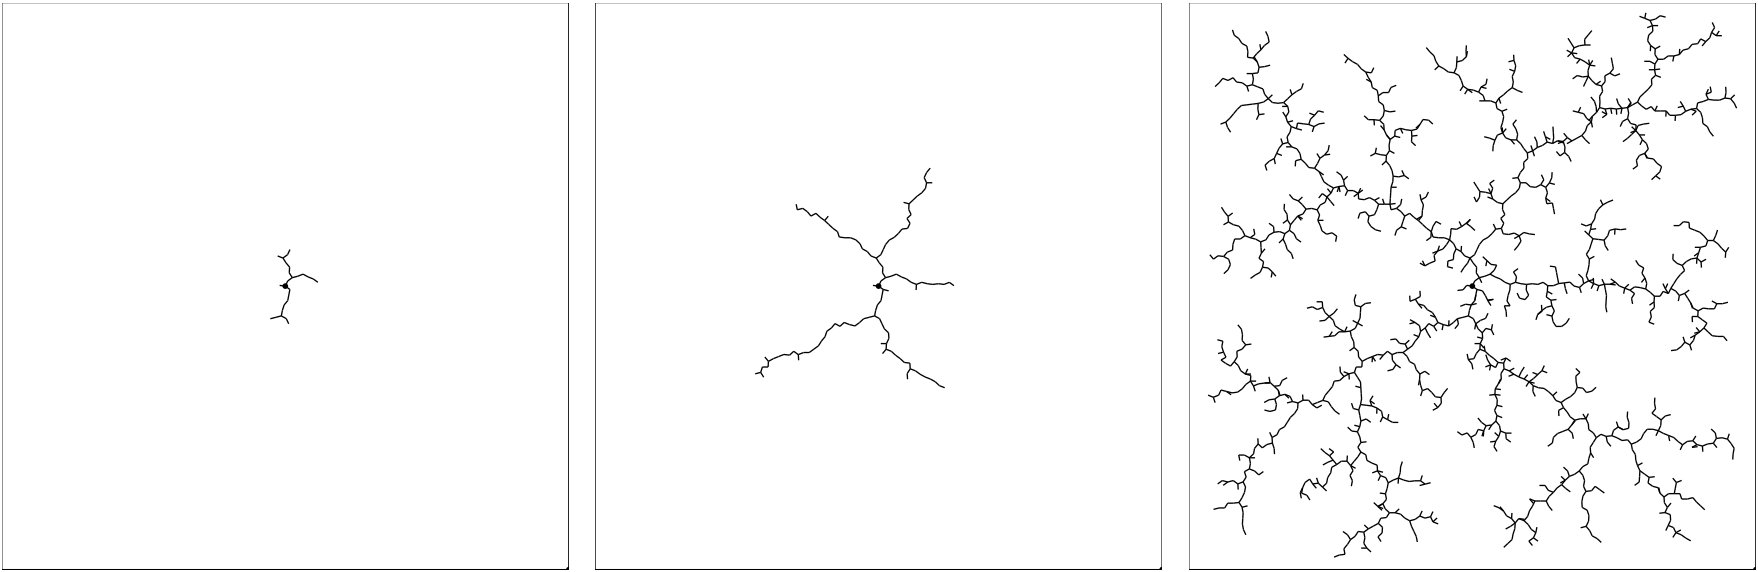
\includegraphics[width=0.75\textwidth]{import/RRT_exploration_tree.png}
	\caption{The RRT algorithm shown expanding in a uniformly random manner. This implementation lacks a goal state. \textbf{Source}: [\citeauthor{Cheng2001}].}
	\label{fig:RRT_treeVanilla}
\end{figure}

One of the advantages of sampling based algorithms over many other methods, including \gls{APF} and A* (which relies on decomposing space into cells) is that it does \textit{not} require an explicit representation of obstacles in C-space [\citeauthor{Karaman2011}]. This is advantageous because such a requirement may lead to excessive computational burden in high \gls{DoF} systems or scenarios with complex environments featuring many obstacles.

Sampling-based methods avoid explicit representation by relying on a collision checking module. This relaxes the completeness criteria, making the algorithms probabilistic complete, as mentioned in Section \ref{sec:planalgo}. In other words, the likelihood of an algorithm returning a path provided that one exist goes to $1$ as the number of samples go to $\infty$.

Another randomized sampling-based method that has seen much use is the \gls{PRM}. \gls{PRM} and \gls{RRT} are fundamentally similar, except \gls{PRM} is a multi-query planner and \gls{RRT} a single-query planner. 

\gls{PRM} first builds up a large number of configuration points in C-space by (mostly) randomly sampling them, without any idea of what the start and goal state could be. A user will then query the \gls{PRM} planner, providing a start and goal state, triggering the planner to start working on creating a path of concatenated straight edges from one connecting node to the other. The first part is called the pre-processing phase, and the second part the query phase [\citeauthor{Kavraki1998}].

Multi-query planners are appropriate when the environment can be assumed to be static, i.e. the environment does not change in terms of the robot or the obstacles. Obviously, any change in the environment would necessitate the reprocessing of the stored points, either by redoing the collision check or discarding them altogether and starting from scratch.

Single-query planners like \gls{RRT} are hence more appropriate in dynamic situations, when the query comes and the points are sampled and a path produced as a response to it online.

\subsubsection{The Algorithm} \label{subsubsec:RRRTAlgo}
	
Assuming that there is a set $\mathcal{V}$ of vertices and a set $\mathcal{E}$ of edges making up graph $\mathcal{G}=(\mathcal{V},\mathcal{E})$; as well as a maximum distance $d$, the algorithm is as follows [\citeauthor{Karaman2011}]:
\begin{enumerate}
	\item Add the initial point $\textbf{p}_{initial}$ to $\mathcal{V}$. $\mathcal{E} = \emptyset$.
	\item Sample $\textbf{p}_{random}$.
	\item Find the $\textbf{p}_{nearest}$ nearest point in $\mathcal{V}$.
	\item Produce a $\textbf{p}_{new}$ such that it is a $d$ distance from $\textbf{p}_{nearest}$ in the direction of  $\textbf{p}_{random}$.
	\item \textbf{If} the line segment between $\textbf{p}_{nearest}$ and $\textbf{p}_{new}$ is collision free: update $\mathcal{V}$ with $\textbf{p}_{new}$, update $\mathcal{E}$ with the line segment. 
	\begin{enumerate}
		\item \textbf{If} $\textbf{p}_{new}$ is the goal state (or in a goal region): \textbf{return} $\mathcal{G}$.
	\end{enumerate}
		\item Return to Step 2.
\end{enumerate}

[\citeauthor{LaValle2006}] suggested that if the $\textbf{p}_{nearest}$ produced in Step 3 lies on an edge between two vertices, the edge should be split up and a new vertex be created on that spot. Furthermore, if $\textbf{p}_{new}$ lies in an obstacle, or if part of the line segment does, the algorithm should travel along the edge to where the line segment enters the obstacle and set a vertex on that boundary ($\textbf{p}_s$ in Figure \ref{fig:RRT_edgetravel}).

\begin{figure}[h]
	\centering
	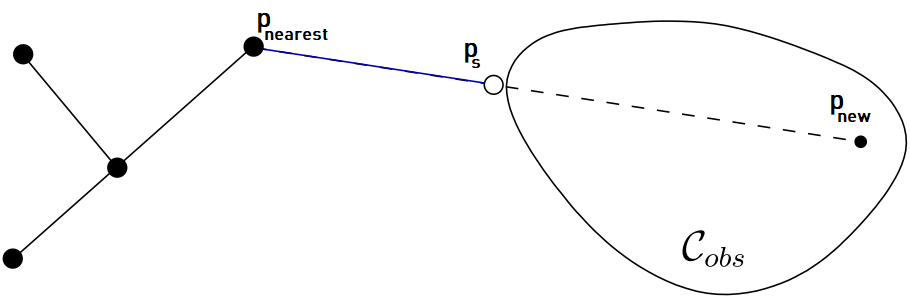
\includegraphics[width=0.55\textwidth]{import/RRT_edgetravel.png}
	\caption{If the $\textbf{p}_{new}$ is in an obstacle region ($\mathcal{C}_{obs}$) it could propose a $\textbf{p}_s$. \textbf{Source}: [\citeauthor{LaValle2006}] with modifications.}
	\label{fig:RRT_edgetravel}
\end{figure}

In Step 5 a collision detection query is made. Considering that it is one of the major focuses of this thesis, it is obviously a very non-trivial step and it will be expounded upon later (e.g., Section \ref{sec:ColliD}).

How $\textbf{p}_{random}$ should be sampled is not completely straightforward either. Section \ref{subsec:Sampling} details how one might bias the sampling.

\subsubsection{Nonholonomic Constraints and Kinodynamics}
A constraint on the $k$ coordinates $\textbf{r}_1, ..., \textbf{r}_k$ can be called holonomic if it is a constraint of the form of,
\begin{equation}
	g_i(\textbf{r}_1, ..., \textbf{r}_k) = 0, i = 1, ..., l.
	\label{eq:holonomic}
\end{equation}
If it is not an equality constraint of this kind it is nonholonomic [\citeauthor{Spong2004}]. An example of a holonomic system would be two particles connected by a rigid beam without mass. Normally, a two particle system would have six \gls{DoF} (two particles capable of three-dimensional translation), but a \gls{DoF} is lost due to the fact that the length between the particles is constant [\citeauthor{Chung2004}]. If a a constraint cannot be expressed in the form of Equation \ref{eq:holonomic} it is nonholonomic, such as constraints given by inequalities are nonholonomic (e.g., a molecule inside of a sphere with radius $\rho$ is subject to $x^2 + y^2 + z^2 < \rho^2$). Mechanical constraints expressed in the following way,
\begin{equation}
	g(r, \dot{r}, \ddot{r}, t) = 0,
	\label{eq:nonholo}
\end{equation}
are nonholonomic if they cannot be reduced to the form of \ref{eq:holonomic}, i.e. if they are nonintegrable [\citeauthor{Chung2004}].

\begin{figure}[h]
	\centering
	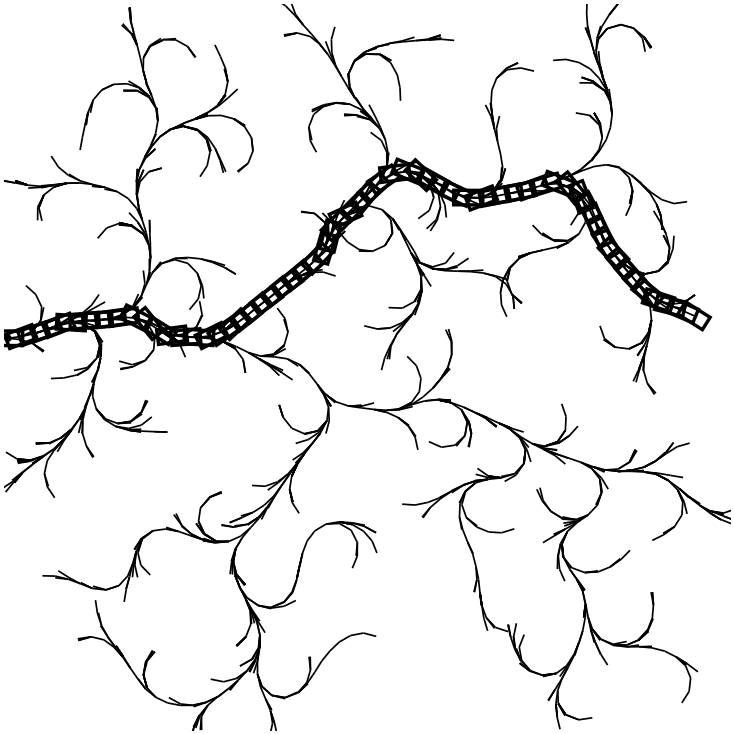
\includegraphics[width=0.3\textwidth]{import/RRT_kinodcar.png}
	\caption{A 5D RRT for a kinodynamic car, that has been projected down to two dimensions. \textbf{Source}: [\citeauthor{LaValle1998}].}
	\label{fig:RRT_kinod}
\end{figure}

In kinodynamic planning, constraints set on the velocity, acceleration, force and torque must be satisfied along with any kinematic goals (e.g., avoiding an obstacle) [\citeauthor{Donald1993}]. Figure \ref{fig:RRT_kinod} shows how an \gls{RRT} tree can be generated that takes into account the kinodynamic properties of a car. A car cannot simply suddenly accelerate to the side, but must roll forward and turn in accordance with its steering system. We can take differential constraints into account by substituting the C-space  with that of a $T(C)$-space, which represents the tangent bundle of the C-space [\citeauthor{LaValle1998}]. An impossible acceleration would thus lie in a forbidden region, which would be returned by the "obstacle detection" module as illegal.



\subsubsection{Sampling} \label{subsec:Sampling}

Figure \ref{fig:RRT_voronoi} shows how the \gls{RRT} algorithm is naturally biased towards exploring the large Voronoi regions (regions of low node density), effectively breaking up the space it is exploring in. This serves as a visual aide in showing how \gls{RRT} is probabilistically complete.

\begin{figure}[h]
	\centering
	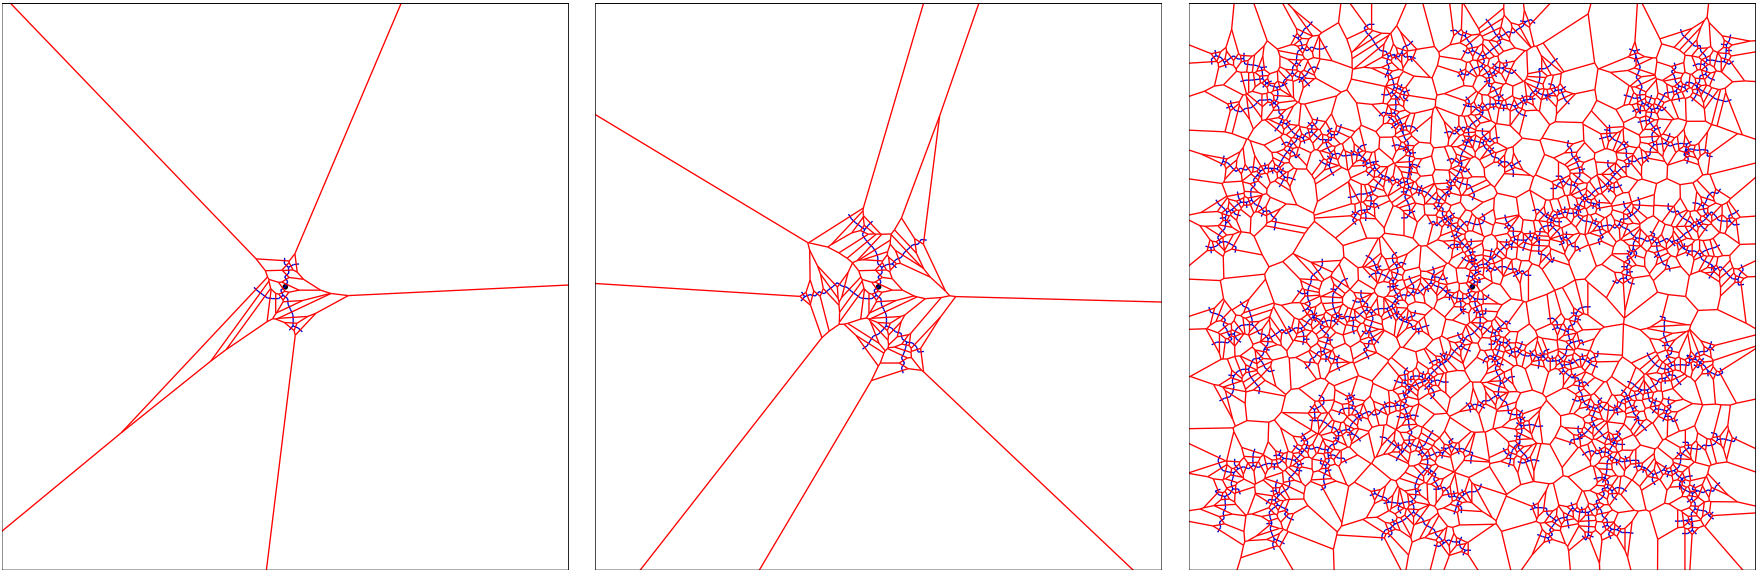
\includegraphics[width=1\textwidth]{import/RRT_voronoi_region.png}
	\caption{The Voronoi regions associated with each uniformly sampled point from Figure \ref{fig:RRT_treeVanilla}. \textbf{Source}: [\citeauthor{Cheng2001}].}
	\label{fig:RRT_voronoi}
\end{figure}

The vanilla \gls{RRT} as it has been mentioned so far is by itself an algorithm made to efficiently explore C-space, but not necessarily to solve planning queries. In fact, \gls{RRT} can have supplementary uses in other algorithms, such as helping to escape local minima [\citeauthor{LaValle2006}] in \gls{APF}, a problem of mentioned in Section \ref{subsubsec:localminima}. 

To make it more suitable, one could grow a tree from an initial configuration $\textbf{p}_{initial}$ and then periodically try to see if it is possible to connect the \gls{RRT} to a $\textbf{p}_{goal}$. One way to achieve this is to do the sample with a $0.01$ probability that $\textbf{p}_{random} = \textbf{p}_{goal}$. and $0.99$ probability that it will be random. $\frac{1}{100}$ has experimentally been shown to prove well [\citeauthor{LaValle2006}] [\citeauthor{Urmson2004}]. Research has gone into ways of biasing the sampling mechanism without compromising the probabilistic completeness of the algorithm. In general, provided that the mechanism will provide a dense sequence of samples with a probability of 1, meaning that the produced graph gets arbitrarily close to any point in space, any nonuniform sampling method is acceptable [\citeauthor{LaValle2006}].

In the field of autonomous driving, [\citeauthor{Link2009}] created a variant of \gls{RRT} called Close-Loop-\gls{RRT}. They integrated the \gls{RRT} algorithm in a control loop controlling an autonomous car. They argued that in structured environments (e.g., an urban environment) sampling purely randomly could result in an big number of wasted samples. Instead, they drew their sample from the controller's input space.

\begin{figure}[h]
	\centering
	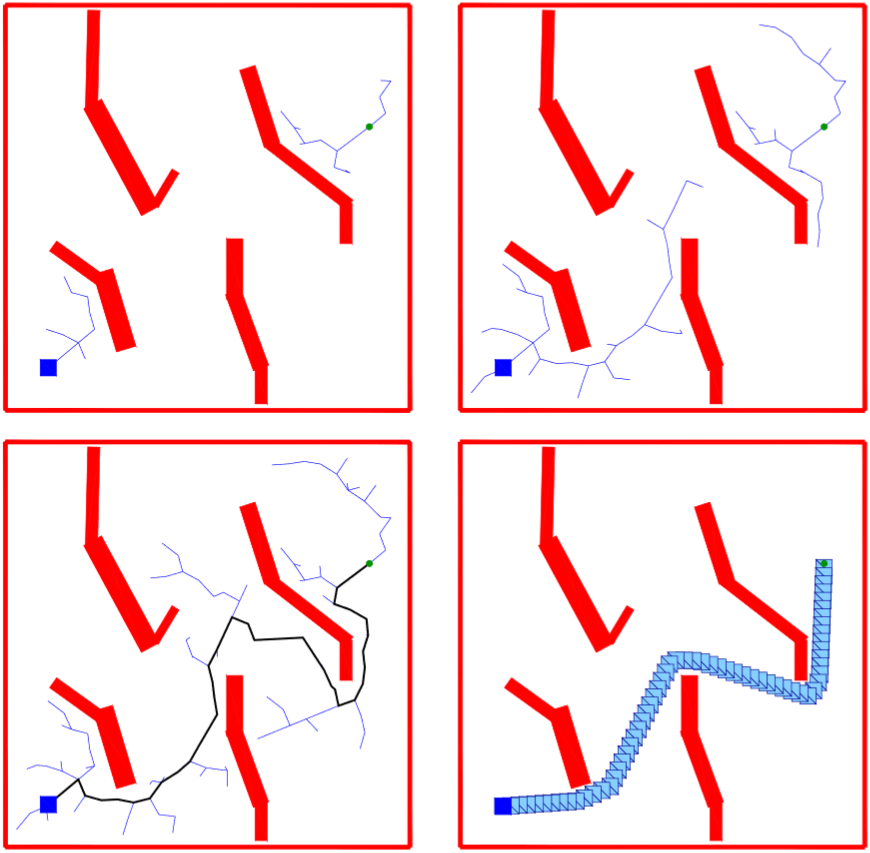
\includegraphics[width=0.45\textwidth]{import/RRT_connect.png}
	\caption{The RRT-connect algorithm. Trees expand from the start and goal node, impeded by the red obstacle regions. \textbf{Source}: [\citeauthor{Kuffner2002}].}
	\label{fig:RRT_connect}
\end{figure}

Variants aiming to help the algorithm converge faster have also been introduced. For example, \gls{RRT}-Connect (shown in Figure \ref{fig:RRT_connect}) works by growing two trees simultaneously, one from the start position and one from the goal [\citeauthor{Kuffner2002}]. The trees work to both explore the areas around them, as well as to grow towards each other using a greedy heuristic.

\subsubsection{Optimality}

\gls{RRT} in its original form is probabilistically complete, but it does not guarantee that the paths produced are in any way optimal. In fact, it has been shown that the solutions the algorithm converges to are almost surely non-optimal (in terms of path length, time cost, etc) [\citeauthor{Karaman2011}]. Thus, variants of the vanilla \gls{RRT} concerned with finding optimal solutions have been presented to help address this problem.

\gls{RRT}* was introduced in [\citeauthor{Karaman2011}] as a way to produce optimal paths from \gls{RRT}, given a cost function. It adds vertices to $\mathcal{V}$ in the same way as \gls{RRT}, as well as consider the nearest points in order to return $\textbf{p}_{nearest}$. The difference is that not all feasible connections will result in new edges being added to $\mathcal{E}$. \gls{RRT}* maintains a tree structure, and will add the new edge (to $\textbf{p}_{new}$) in a path that will result in the lowest path cost. Also, new edges from the nearest vertices to $\textbf{p}_{new}$ are examined, and if lower cost paths can be found through $\textbf{p}_{new}$ then the algorithm will create new edges and prune away old ones.
 
One limitation of \gls{RRT}* is that it is only applicable to systems with simple dynamics, due to relying on the ability to connect any pair of states with an optimal trajectory. [\citeauthor{Webb2012}] introduced Kinodynamic \gls{RRT}* to deal with this, by using a fixed-final-state-free-final-time optimal control formulation.

Transition-based \gls{RRT}, or T-\gls{RRT}is another improvement introduced in [\citeauthor{Jaillet2008}]. As the name suggest, it makes use of transition tests to judge whether to accept or reject a new potential state, a concept inspired from stochastic optimization (e.g., Monte Carlo optimization) that was developed in order to find global optima in very complex function spaces. T-\gls{RRT} also relies on a notion of a minimal work path to evaluate path costs.

\begin{figure}[h]
	\centering
	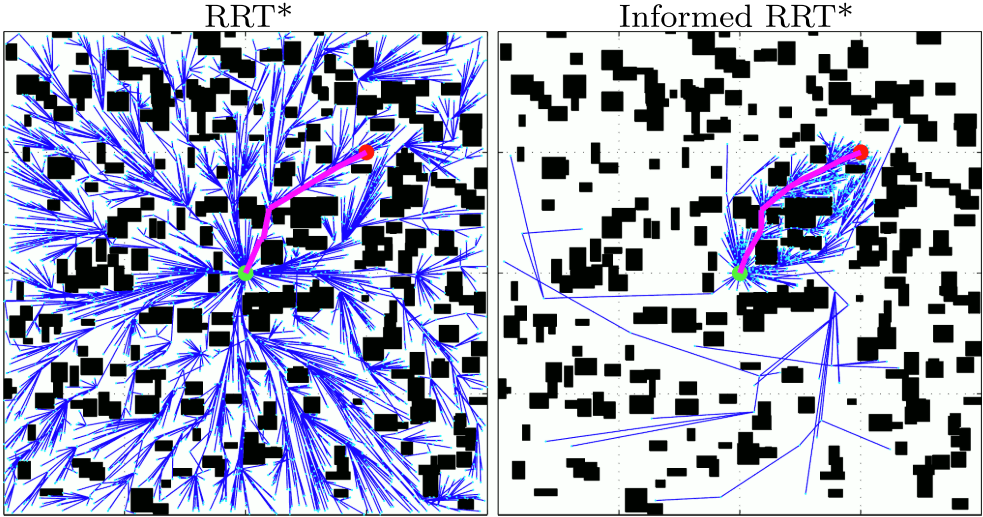
\includegraphics[width=0.65\textwidth]{import/RRT_starvsinformed.png}
	\caption{A comparison between RRT* and Informed RRT*. \textbf{Source}: [\citeauthor{Gammell2014}].}
	\label{fig:RRT_optimal_comp}
\end{figure}

Informed \gls{RRT}* was presented in [\citeauthor{Gammell2014}] as an improvement on \gls{RRT}*. Informed \gls{RRT}* incorporates search heuristics in order to avoid having to find the optimal path from \textit{every} state, as \gls{RRT}* does. Figure \ref{fig:RRT_optimal_comp} shows \gls{RRT}* and Informed \gls{RRT}* finding equivalent (optimal) cost solutions to a goal. In that specific experiment, Informed \gls{RRT}* required $\frac{1}{8}$ of the time to reach the same path. Informed \gls{RRT}* narrows down the search on an ellipsoidal informed subset of the state space once an initial solution is found.

\section{Collision Detection}\label{sec:ColliD}

This section is dedicated to listing various methods for collision detection.

\subsection{Bounding Box Methods} \label{subsec:BBM}

\textit{Bounding Box methods} refers to methods that work on the principle of enclosing objects in boxes and then operating on or with those boxes. 

The boxes are meant to be minimally encompassing, in the sense that they cover as little beyond their inner objects as possible, along the axes they are defined on. For the 3D case, the box can be formulated as:
\begin{equation}
\mathcal{B} = \{x_{min}, x_{max}, y_{min}, y_{max}, z_{min}, z_{max}\}.
\end{equation}
$\mathcal{B}$ can be set by sorting through the set of points comprising the object it is to enclose and setting the parameters accordingly. This is the basis for \gls{AABB}.

\subsubsection{Axis-Aligned Bounding Boxes}
\gls{AABB} is a simple bounding box method that relies on the Cartesian coordinate axes of the overall world frame. Checking if a point $\textbf{P}$ is within bounding box $\mathcal{B}$ is as simple as checking that all of the following inequalities are true:
\begin{equation}
\begin{Bmatrix}
\mathcal{B}_{x_{min}} \\ \mathcal{B}_{y_{min}} \\ \mathcal{B}_{z_{min}}
\end{Bmatrix}
\leq
\begin{pmatrix}
\textbf{P}_x \\ \textbf{P}_y \\ \textbf{P}_z
\end{pmatrix}
\leq
\begin{Bmatrix}
\mathcal{B}_{x_{max}} \\ \mathcal{B}_{y_{max}} \\ \mathcal{B}_{z_{max}}
\end{Bmatrix}.
\end{equation}

It is simple to extend this to checking if two bounding boxes, cuboids $\mathcal{B}$ and $\mathcal{C}$, are intersecting. In such a case, the following inequalities hold true:

\begin{equation}
\begin{Bmatrix}
\mathcal{B}_{x_{min}} \\ \mathcal{B}_{y_{min}} \\ \mathcal{B}_{z_{min}}
\end{Bmatrix}
\leq
\begin{Bmatrix}
\mathcal{C}_{x_{max}} \\ \mathcal{C}_{y_{max}} \\ \mathcal{C}_{z_{max}}
\end{Bmatrix}
\wedge
\begin{Bmatrix}
\mathcal{B}_{x_{max}} \\ \mathcal{B}_{y_{max}} \\ \mathcal{B}_{z_{max}}
\end{Bmatrix}
\geq
\begin{Bmatrix}
\mathcal{C}_{x_{min}} \\ \mathcal{C}_{y_{min}} \\ \mathcal{C}_{z_{min}}
\end{Bmatrix}
\end{equation}



%\begin{lstlisting}
%	def isPointInsideAABB(B, point):
%		return ((point.x >= B.xmin && point.x <= B.xmax) &&
%		(point.y >= box.minY && point.y <= box.maxY) &&
%		(point.z >= box.minY && point.z <= box.maxZ))
%\end{lstlisting}


\subsubsection{Oriented Bounding Boxes}
\gls{OBB} is similar to \gls{AABB}, except instead of using the world frame it makes use of a local coordinate system associated with the local object itself, or any arbitrarily chosen orientation [\citeauthor{VanDenBergen1998}]. 

In cases where the object just so happens to not expand in the directions of the Cartesian coordinate axes $x$, $y$ or $z$, an \gls{AABB} will be encapsulating an unnecessary amount of empty space, returning false positives to collision queries. For example, a $1^3$ volume units cube rotated $\frac{\pi}{4}$ radians will need a $\sqrt{2}^3\approx 2.83$ volume units cube to encompass it. The rotated cube would only be occupying $\frac{\sqrt{2}^3 - 1^3}{\sqrt{2}^3} \approx 0.65\%$ of the space. If the axes drawing the bounding box could rotate along with it, $100\%$ of the space would still be used.

This freedom comes at the cost of \textit{storage} space. An \gls{OBB} is represented using $15$ scalars: a $3 \times 3$ orientation matrix, $3 \times 1$ vector for position and $3$ variables for extent [\citeauthor{VanDenBergen1998}]. Meanwhile, an \gls{AABB} requires only $6$, as shown earlier.

The \textit{Separating Axis Theorem} was introduced in [\citeauthor{Gottschalk1996}], and is a method used to efficiently check overlap between two \gls{OBB}s. It is based on the fact that two disjoint convex polytopes in 3D space can always be separated by a plane parallel to either an edge from each polytope, or a face of either polytope. Thus, two convex polytopes are disjoint only if there exists such a separating axis orthogonal to an edge of either polytope, or orthogonal to a face form each polytope. As such, 15 candidate separating axes need to be tested, stemming from the six faces of the \gls{OBB} and the nine pairwise combination of edges. 

\begin{figure}[h]
	\centering
	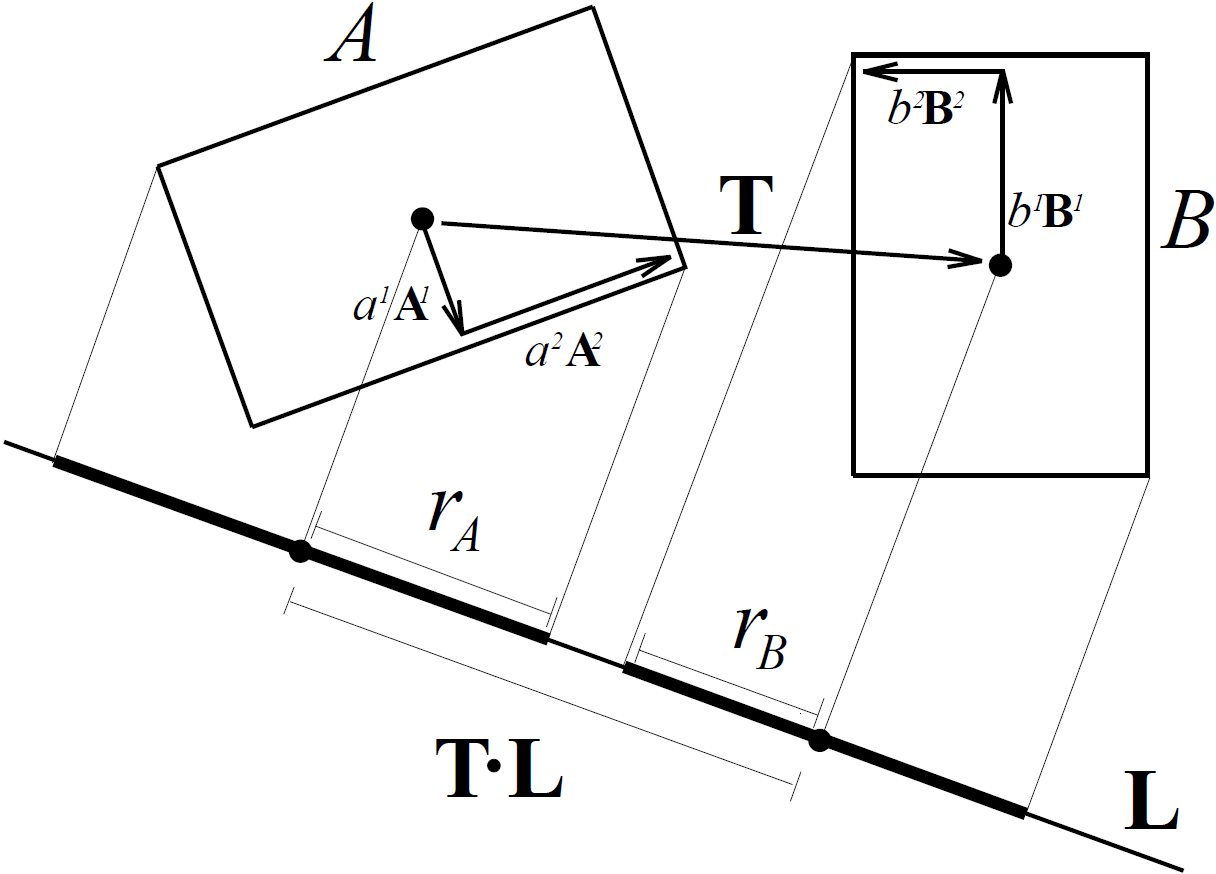
\includegraphics[width=0.43\textwidth]{import/OBB_sepaxis.png}
	\caption{Two OBB $A$ and $B$, along with a separating axis $\textbf{L}$. \textbf{Source}: [\citeauthor{Gottschalk1996}].}
	\label{fig:OBB_sepaxis}
\end{figure}


If the \gls{OBB} do not overlap, a separating axis will exist and it will be one of those 15 axes listed. If the \gls{OBB} are not disjoint, no separating axis will exist.

Figure \ref{fig:OBB_sepaxis} illustrates this concept. In that case $\textbf{L}$ constitutes a separating axis as the projected versions of $A$ and $B$ do not overlap along it. The projections $\textbf{r}_A$ and $\textbf{r}_B$ are the sum of their respective radii ($a^1, a^2, b^1, b^2$) in their respective axes unit vectors ($\textbf{A}^1, \textbf{A}^2, \textbf{B}^1, \textbf{B}^2$) projected onto the separating axis $\textbf{L}$.

\subsubsection{Bounding Volume Hierarchy}

For more complex environments, one method of speeding up collision detection queries is to structure the bounding volumes into a tree structure [\citeauthor{Haverkort2004}]. Objects are recursively wrapped into bounding volumes that form leaf nodes on the tree, as modes are grouped in small sets and enclosed into larger bounding volumes represented as their parent in the tree. When a collision detection query is made, sibling nodes are pairwise checked for collision from top to bottom until a collision is detected. 

\begin{figure}[h]
	
	\dirtree{%
		.1 \textbf{0:}World.
		.2 \textbf{1:}Character A.
		.3 \textbf{2:}Upper Body.
		.4 \textbf{3:}Right Half Torso.
		.5 \textbf{4:}Right Arm.
		.6 \textbf{5:}Right Forearm.
		.7 \textbf{6:}Right Hand.
		.8 \textbf{7:}Right Thumb.
		.7 \textbf{6:}-------.
		.6 \textbf{5:}------.
		.5 \textbf{4:}-----.
		.4 \textbf{3:}----.
		.3 \textbf{2:}---.
		.2 \textbf{1:}Character B.
		.3 \textbf{2:}---.
	}
	\caption{A bounding volume hierarchy organizing objects into a tree structure. Two characters inhabit the world, with an anatomy defined in the tree nodes. Dashes are used for brevity, to avoid having to list all child nodes at each level.}
	\label{fig:BVH_tree}
\end{figure}

Take as an example a game containing a world inhabited by two characters, A and B, as shown in Figure \ref{fig:BVH_tree}. The naive approach would be to check collisions between all level 7 bounding boxes, of which there are $2^7 = 128$. Checking every bounding box on level $n$, all with each other, would require $O(2^{n^2})$ checks. A better approach would be to move from the top-most node down, and only doing checks on child nodes of those whose parents are intersecting.

\subsection{Gilbert-Jonhson-Keerthi Distance Algorithm}

The \gls{GJK} algorithm is an algorithm used for calculating minimum distances between a pair of convex sets [\citeauthor{Gilbert1987}]. The algorithm was designed to be most efficient for 3D space, where the convex sets are polytopes defined by their vertices. The algorithm works iteratively to find the distance, but was shown to terminate in a finite number of steps in such a scenario, growing linearly in the total number of vertices associated with the two polytopes. 

An extended version for non-polytopal convex objects (e.g., cones or cylinders) was presented in [\citeauthor{Gilbert1990}]. That version, while fast does not converge in finite time. But it was shown that by setting an effective stopping condition, numerical solutions with guaranteed accuracy could be computed. Extensive numerical experiments supported this claimed efficiency.

The distance between objects \textit{A} and \textit{B}, represented by a set of points $\mathcal{K}_A$ and $\mathcal{K}_B$, is given by the following,
\begin{equation}
d(\mathcal{K}_A,\mathcal{K}_B) = \min \{|\textbf{p}_A - \textbf{p}_B|^2 : \textbf{p}_A \in \mathcal{K}_A, \textbf{p}_B \in \mathcal{K}_B,  \mathcal{K}_A, \mathcal{K}_B \subset \mathbb{R}^m\}.
\end{equation}
Provided that $\mathcal{K}_A$ and $\mathcal{K}_B$ are compact sets, i.e. containing all their limits points and having all points $\textbf{p}_*$ lie in a fixed distance of each other, such a minimum distance will exist [\citeauthor{Gilbert1987}].

\subsubsection{Support Mapping Functions}

\gls{GJK} relies on support mapping functions to describe the convex sets, reducing the problem to computing the distance between one object to the origin [\citeauthor{Lindemann2009}]. A support mapping function $s_A(\textbf{v})$ of a convex set $\mathcal{K}_A$ maps a vector $\textbf{v}$ to a specific point $\textbf{p}_A$ known as the \textit{support point}. The support point, $\textbf{p}_A$, is the point that is located on the most extreme edge point along the boundary of $\mathcal{K}_A$ in the direction of the vector $\textbf{v}$ [\citeauthor{Lindemann2009}], fulfilling the following equation,

\begin{equation}
\textbf{v} \cdot s_A(\textbf{v}) = \max\{\textbf{v}\cdot \textbf{p}_A : \textbf{p}_A \in \mathcal{K}_A\}.
\end{equation}

For polytopes, this can be calculated in linear time in regards to the number of vertices, and if frame coherence is used it could potentially be reduced to almost constant time. This could be done by maintaining an adjacency graph of the vertices for the polytope, and is also known as \textit{hill climbing} [\citeauthor{VanDenBergen1999}]. Specific convex sets can have support functions that are particularly well suited for them. For example, the following support function for a circle or sphere returns the support point automatically [\citeauthor{Lindemann2009}]:
\begin{equation}
s_A(\textbf{v}) = c_A + r_A\cdot\frac{\textbf{v}}{||\textbf{v}||},
\end{equation}
where $c_A$ is the center of the circle or sphere and $r_A$ the radius. Refer to [\citeauthor{VanDenBergen1999}] for examples of more support functions.

Support functions can thus be calculated easily, making \gls{GJK} reliable and fast. Complicated objects can be disassembled into primitives and then have the calculations performed using the sub-parts.

\subsubsection{Minkowski Difference}

Another point of theory necessary to understand the \gls{GJK} algorithm is that of the Minkowski sum operation [\citeauthor{Gilbert1987}]. It is defined for general $m$-dimensional cases as the following,
\begin{equation}
\mathcal{K}_C = \mathcal{K}_A \pm \mathcal{K}_B = \{\textbf{p}_A \pm \textbf{p}_B : \textbf{p}_A \in \mathcal{K}_A, \textbf{p}_B \in \mathcal{K}_B, \mathcal{K}_A, \mathcal{K}_B \subset \mathbb{R}^m \}.
\end{equation}
In other words, every point in $\mathcal{K}_B$ is added (or subtracted) to every point in $\mathcal{K}_A$, resulting in a new set of points $\mathcal{K}_C$. Note that this operation can result in duplicates $\textbf{p}_C$, so the cardinality of $\mathcal{K}_C$ is always equal to or less than that of $\mathcal{K}_A$ and $\mathcal{K}_B$.

\begin{figure}[h]
	
	\begin{minipage}[t]{1\textwidth}
		\centering
		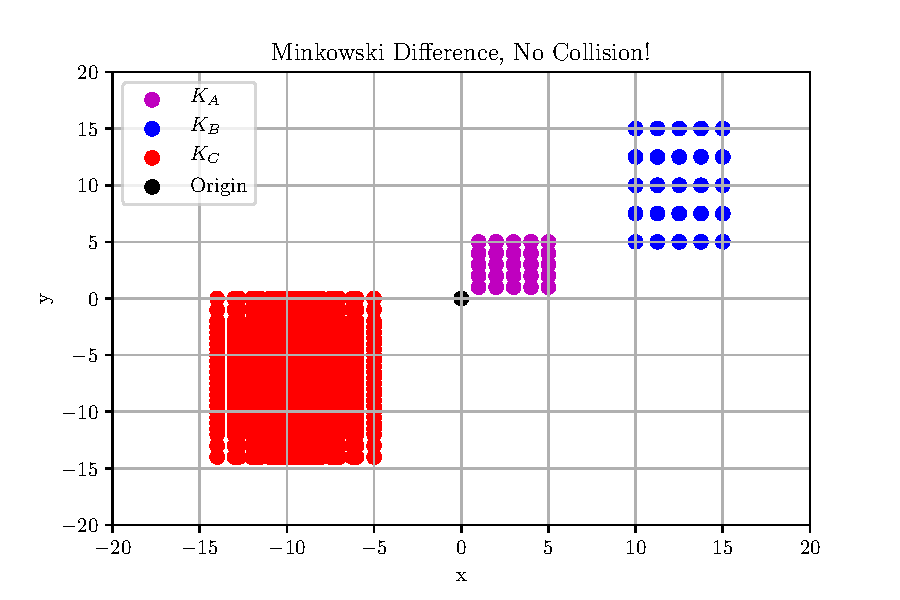
\includegraphics[scale=0.45]{import/No_Collision.pdf}
	\end{minipage}

	\begin{minipage}[t]{1\textwidth}
		\centering
		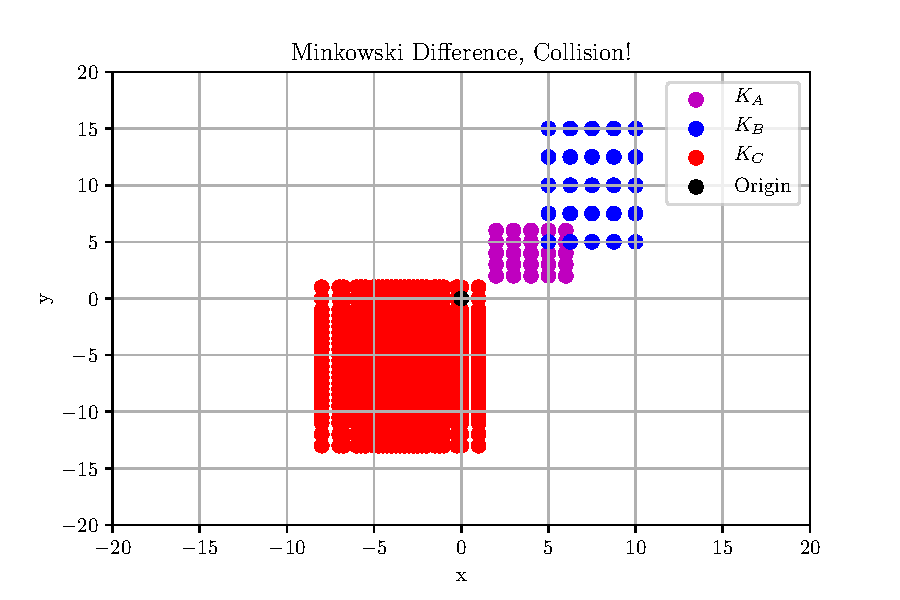
\includegraphics[scale=0.45]{import/Collision.pdf}
	\end{minipage}
	\caption{Minkowski difference being taken on sets $\mathcal{K}_A$ and $\mathcal{K}_B$ resulting in $\mathcal{K}_C$.}
	\label{fig:minkow}
\end{figure}
%{\color{magenta}}, {\color{blue}, {\color{red} 
The Minkowski sum, or rather the Minkowski \textit{difference} specifically, is the key to \gls{GJK}, as it can be shown that the shortest distance difference between $\mathcal{K}_A$ and $\mathcal{K}_B$ is equal to the closest distance between $\mathcal{K}_C$ and the origin [\citeauthor{Lindemann2009}]. The support mapping functions can similarly be calculated as,
\begin{equation}
s_C(\textbf{v}) = s_{A\pm  B}(\textbf{v}) = s_A(\textbf{v})\pm s_B(\pm\textbf{v}).
\end{equation}
Thus, if two objects are intersecting (i.e., colliding), the $\textbf{p}_C$ closest to the origin will be the origin itself. In other words, if the origin is a part of the Minkowski difference $\mathcal{K}_C$, $\mathcal{K}_A$ and $\mathcal{K}_B$ are in collision. This is shown in Figure \ref{fig:minkow}, where in the upper scenario the origin is not a point in $\mathcal{K}_C$ but in the lower scenario it is, due to the intersection around $(5,5)$.

\subsubsection{The Iterative Algorithm} \label{subsubsec:GJKiter}

For the purposes of this algorithm, for a given set $\mathcal{A}$ and given set of vertices $\mathcal{W}$, $\textbf{v}(\mathcal{A})$ is meant to return the point closest to the origin in set $\mathcal{A}$, and $CH(\mathcal{W})$ refers to the convex hull spanned by the set of vertices $\mathcal{W}$. 

\begin{figure}[h]
	\centering
	\begin{minipage}[h]{0.3\textwidth}
		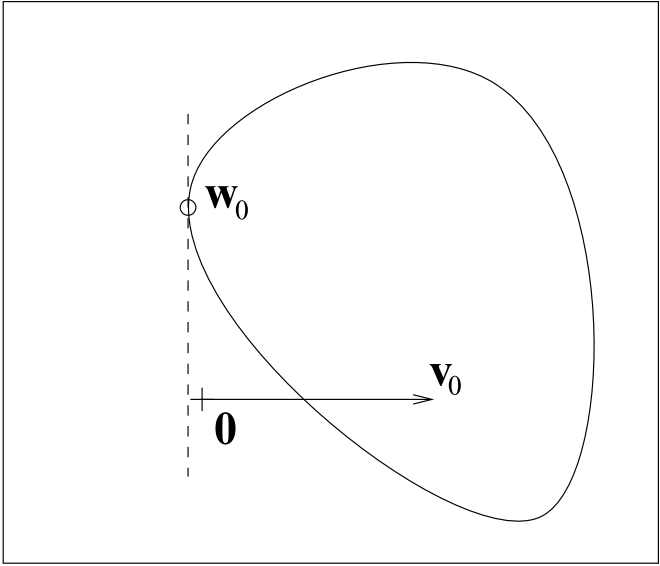
\includegraphics[width=1\textwidth]{import/GJK_1.png}
		\subcaption{$i=0,\mathcal{W} = \emptyset$}
		\label{fig:GJK1}
	\end{minipage}
	\hspace{1cm}
	\begin{minipage}[h]{0.3\textwidth}
		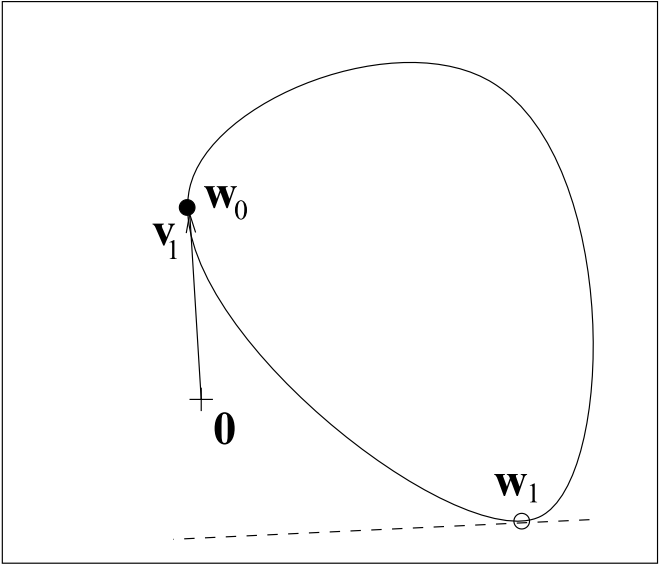
\includegraphics[width=1\textwidth]{import/GJK_2.png}
		\subcaption{$i=1,\mathcal{W} =\{\textbf{w}_0\}$}
		\label{fig:GJK2}
	\end{minipage}
	\begin{minipage}[h]{0.3\textwidth}
		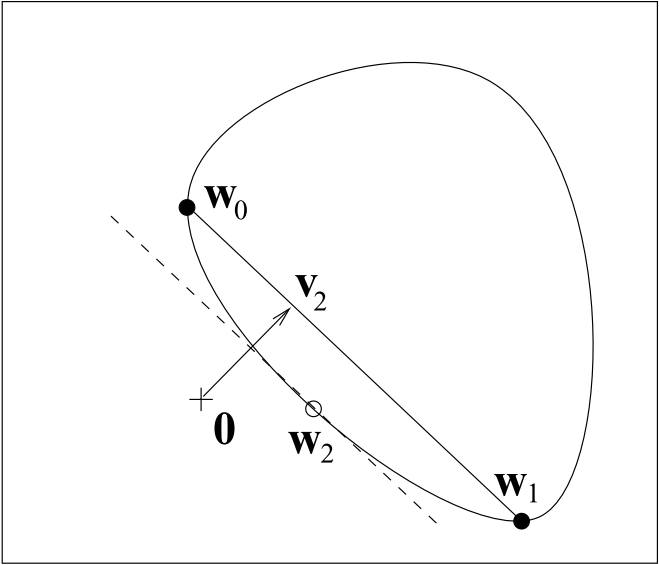
\includegraphics[width=1\textwidth]{import/GJK_3.png}
		\subcaption{$i=2,\mathcal{W} =\{\textbf{w}_0, \textbf{w}_1\}$}
		\label{fig:GJK3}
	\end{minipage}
	\hspace{1cm}
	\begin{minipage}[h]{0.3\textwidth}
		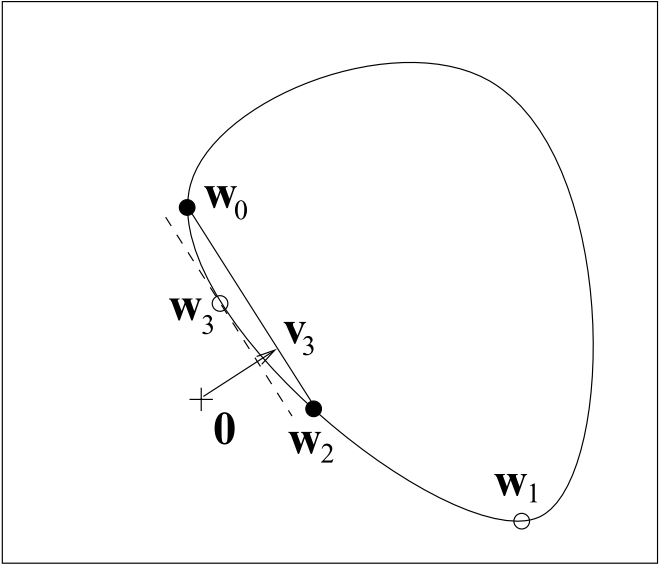
\includegraphics[width=1\textwidth]{import/GJK_4.png}
		\subcaption{$i=3,\mathcal{W} =\{\textbf{w}_0, \textbf{w}_2\}$}
		\label{fig:GJK4}
	\end{minipage}
	\caption{Four iterations of the GJK algorithm. Note that the origin is not part of the set. \textbf{Source}: [\citeauthor{VanDenBergen1999}].}
	\label{fig:GJK_Algo}
\end{figure}

As mentioned, the \gls{GJK} works iteratively. It produces a simplex in $K_C$ that is closer and closer to the origin in each step. The simplex is composed of a set of vertices, stored in $\mathcal{W}_i$, where $i$ represents the $i$th iteration of the algorithm. The simplex computed in each iteration has a convex hull, on which lies $\textbf{v}_i$ defined as the point closest to the origin ($\textbf{v}_i = \textbf{v}(CH(W_i))$) in iteration $i$. The algorithm is then as follows [\citeauthor{Lindemann2009}]:

\begin{enumerate}
	\item Initialization step:
	\begin{enumerate}
		\item Let i = 0.
		\item Define the simplex set $\mathcal{W}_0 = \emptyset$.
		\item Let $\textbf{v}_0$ be an arbitrary point within $K_C$.
	\end{enumerate}
	\item Compute the support point $\textbf{w}_i = s_C(-\textbf{v}_i)$ in direction $-\textbf{v}_i$.
	\item \textbf{If} $\,\textbf{w}_i$ is no more extreme than $\textbf{v}_i$ in direction $-\textbf{v}_i$: \textbf{return} $||\textbf{v}_i||$.
	\item \textbf{Else}: add $\textbf{w}_i$ to the current simplex set $\mathcal{W}_i$.
	\item Compute $\textbf{v}_{i+1} = \textbf{v}(CH(W_i \cup \{\textbf{w}_i\}))$.
	\item Make $\mathcal{W}_{i+1}$ the smallest convex subset of  $\mathcal{W}_i\, \cup \, \{\textbf{w}_i\}$ still containing $\textbf{v}_{i+1}$.
	\item $i_{++}$, go to Step 2.
\end{enumerate}

Figure \ref{fig:GJK_Algo} presents four iterations of the algorithm for the reader's convenience.

In Step 3 the function will produce the distance to the origin, for which a value of 0 (or $||\textbf{v}_i|| < \epsilon$, for a small $\epsilon$) would imply collision.

Step 5 computes $\textbf{v}_{i+1}$, but this is not exactly a trivial task. Originally \textit{Johnson's Distance Subalgorithm} [\citeauthor{Gilbert1987}] was used, it searches all simplex subsets and solves systems of linear equations for each subset recursively [\citeauthor{Ericson2004}]. Advances over time have however made it obsolete [\citeauthor{Lindemann2009}].

One alternative algorithm was provided in [\citeauthor{Cameron2002}], which also makes use of support mapping functions and the aforementioned hill climbing method. It buffers the support point from the last iteration, and then checks its neighboring vertices first in the current iteration. For larger convex hulls it brought dramatic improvements.

Another alternative method was presented in [\citeauthor{Ericson2004}] is mathematically equivalent to the \textit{Johnson's Distance Subalgorithm}, but relies instead on a geometrical approach that the author claims to be more intuitive. It relies on dividing the space into Voronoi regions defined by the points and the edges, as seen in Figure \ref{fig:GJK_E}.
\begin{enumerate}
	\item If the origin lies in a vertex's region, that vertex is the closest point.
	\item If the origin lies in an edge's region, the closest point is somewhere on that edge. The closest point can be calculated using the orthogonal projection on that edge (which is vector between two points).
	\item If the origin is in neither a vertex region or edge region, it must be in the face region.
\end{enumerate}


\begin{figure}
	\centering
	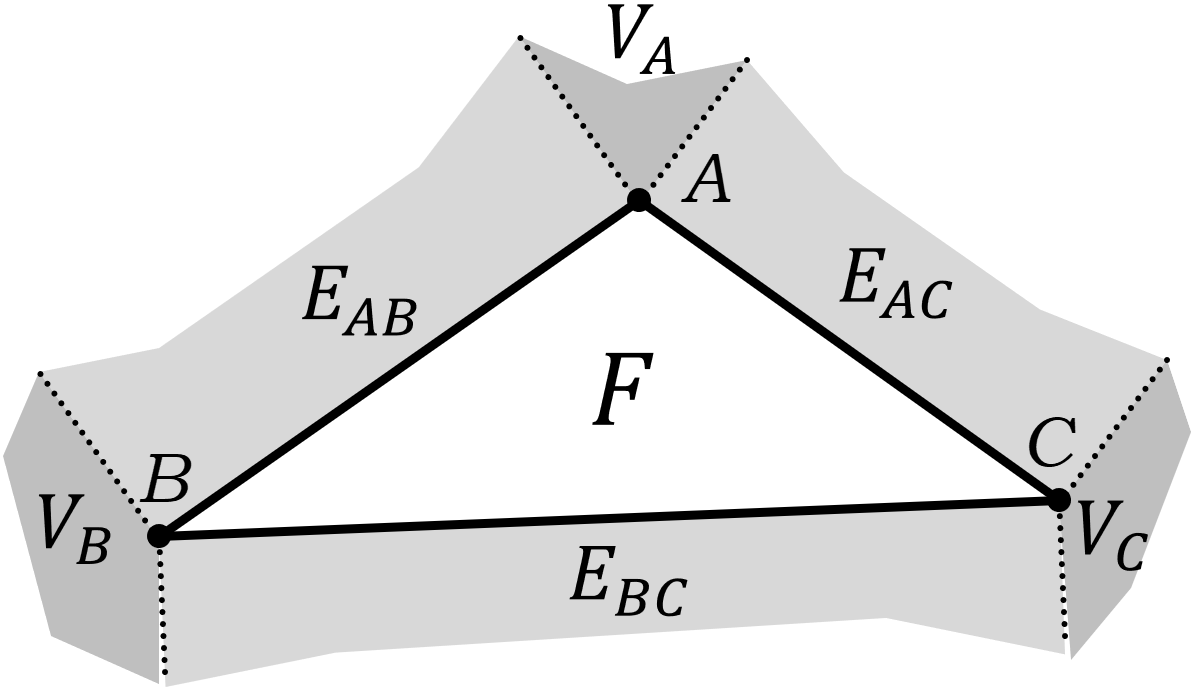
\includegraphics[width=0.55\textwidth]{import/GJK_Ericson.png}
	\caption{An illustration of convex hull with face $F$, the vertices $\textbf{A} = \textbf{q}_1$, $\textbf{B} = \textbf{q}_2$ and $\textbf{C} = \textbf{q}_3$, as well as the Voronoi regions (\textbf{E} for edge, \textbf{V} for vertex) $\textbf{E}_{AB}, \textbf{E}_{AC}, \textbf{E}_{BC}, \textbf{V}_A, \textbf{V}_B$ and  $\textbf{V}_C$. \textbf{Source}: [\citeauthor{Ericson2004}]. }
	\label{fig:GJK_E}
\end{figure}
%{\color{yellow}\,

It applies to the 2D scenario of finding intersecting polytopes, but can be generalized to be used in 3D. In 3D, for example, a point could exist above or below the triangle \textit{F}, in addition to being perfectly in its plane.

%Regarding Step 6, the simplifying of $\mathcal{W}_{i+1}$ is done by expressing $\textbf{v}_{i+1}$ as a convex combination of the vertices in $\mathcal{W}_{i}$, expressed as,
%\begin{equation}
%\textbf{v}_{i+1} = \sum_{k=1}^K \alpha_k \textbf{q}_k, \, \alpha_k \geq0 \, \forall k\texttt{},  \sum_{k=1}^K \alpha_k = 1,
%\end{equation}
%where K is the number of vertices in $\mathcal{W}_i$, and $\textbf{q}_i$ the $k$th vertex element in $\mathcal{W}_i$. Carathéodory proved [\citeauthor{Rockafellar1970}] that provided that $\textbf{v}_{i+1}$ is part of the convex hull in $\mathbb{R}^m$, it is possible to express it with $m+1$ many non-zero  $\alpha_k$ values (with the rest as $0$). 

%\subsubsection{Enhanced GJK}


\subsection{Superquadrics}

%As mentioned in Section \ref{subsec:backg}, 
\gls{SQ} are a family of 3D geometric shapes. These shapes are actually surfaces obtained by taking the spherical product of two 2D curves, specifically that of the superellipse presented in its parametric form: 
\begin{equation}
\textbf{s}(\theta) = \begin{bmatrix}
a\,cos^\epsilon\,\eta \\
b\,sin^\epsilon\,\eta
\end{bmatrix}, \hspace{0.5cm}
-\pi \leq \theta \leq \pi,
\label{eq:SuperEllipse}
\end{equation}
or, in its implicit form,
\begin{equation}
\left(\frac{x}{a}\right)^\frac{2}{\epsilon} + \left(\frac{y}{b}\right)^\frac{2}{\epsilon} = 1.
\end{equation}
Note that in the parametric form, taking the exponentiation of the trigonometric functions with $\epsilon$ is defined as a signed power function, such that $cos^\epsilon \theta = sign(cos\theta)|cos\theta|^\epsilon$ and similarly for the sine equivalent.

By taking the spherical product [\citeauthor{H.Barr1981}] of a pair of superellipses, a \textit{superellipsoid} can be obtained:
\begin{multline}
\begin{pmatrix}
x \\ y \\ z
\end{pmatrix} = s_1(\eta) \otimes s_2(\omega) = \begin{bmatrix}
cos^{\epsilon_1}\eta \\ a_3\,\,sin^{\epsilon_1}\eta
\end{bmatrix} \otimes
\begin{bmatrix}
a_1\,cos^{\epsilon_2}\omega \\ a_2\,sin^{\epsilon_2}\omega
\end{bmatrix} = \\  
\begin{bmatrix}
a_1\,cos^{\epsilon_1}\eta\,cos^{\epsilon_2}\omega \\ 
a_2\,cos^{\epsilon_1}\eta\,sin^{\epsilon_2}\omega \\
a_3\,sin^{\epsilon_1}\eta
\end{bmatrix}, \hspace{0.5 cm} \begin{matrix}
-\pi/2 \leq \eta \leq \pi/2 \\
-\pi \leq \omega \leq \pi
\end{matrix}.
\label{eq:SQparam}
\end{multline}
Geometrically, $s_1(\eta)$ is a horizontal curve that is vertically modulated by $s_2(\omega)$. Angle $\eta$ can be seen as a north-south parameter (not unlike latitude), and $\omega$ corresponds to an east-west parameter (like longitude) [\citeauthor{H.Barr1981}]. The dimension parameters $a_1, a_2, a_3$ scale the spherical product in the respective axes. The shape parameters $\epsilon_1$ and $\epsilon_2$ are also known as the squareness parameters, associated with the north-south and east-west directions respectively. They can be used to pinch, round and square off the shape. 

Cuboids are produced when $\epsilon_1 < 1$ and $\epsilon_2 < 1$, cylindroids when $\epsilon_2 \sim 1$ and $\epsilon_1 < 1$ and pillow-shapes when $\epsilon_1 \sim 1$ and $\epsilon_2 < 1$. When either $\epsilon_1$ or $\epsilon_2$ are greater than 2 pinched shapes are produced, and flat-beveled shapes are produced when either $\epsilon_1 = 2$ or $\epsilon_2 = 2$.

The implicit function for this \textit{superellipsoid} can be written as follows,
\begin{equation}
\left(\left(\frac{x}{a_1}\right)^{\frac{2}{\epsilon_2}} + \left(\frac{y}{a_2}\right)^{\frac{2}{\epsilon_2}} \right)^{\frac{\epsilon_2}{\epsilon_1}} + \left(\frac{z}{a_3}\right)^\frac{2}{\epsilon_1} = F_E(\textbf{P}, \mathbf{\Lambda}).
\label{eq:F}
\end{equation}
where $\textbf{P}$ refers to the point $(x,y,z)^T$ and $\mathbf{\Lambda}_5$ the parameters $a_1, a_2, a_3, \epsilon_1, \epsilon_2$. Refer to [\citeauthor{Jaklic2000}] for the details of the conversions between the parametric forms and implicit forms of the respective shapes.

All the points $P$ that satisfy $F=1$ lie on the surface. If a point results in $F < 1$ or $F > 1$ then the point lies inside or outside of the surface respectively. Because the implicit function divides 3D space into three distinct regions (inside, outside, surface boundary), another word for it is \textit{inside-outside} function. 

\begin{figure}[h]
	\centering
	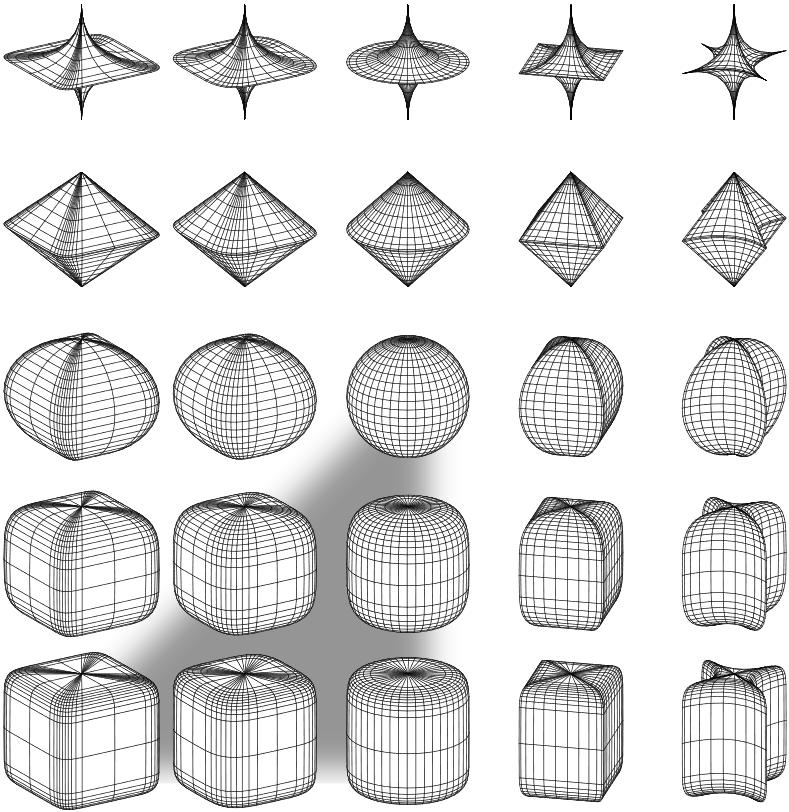
\includegraphics[width=0.35\textheight]{import/SQ_ellipsoids}
	\caption{SQ (superellipsoidals) drawn, for constant $a_1, a_2, a_3$ but varying $\epsilon_1$ (increasing in the figure's $y$-axis) and $\epsilon_2$ (increasing in the figure's $x$-axis). $\epsilon_1,\epsilon_2 = \{\frac{1}{4}, \frac{1}{2}, 1, 2, 4\}$. \textbf{Source}: [\citeauthor{Kindlmann2004}].}
	\label{fig:SQ_ellipsoids}
\end{figure}

A range of superellipsoidal \gls{SQ} have been plotted using Equation \ref{eq:SQparam} in Figure \ref{fig:SQ_ellipsoids}.

\subsubsection*{Non-Superellipsoidal Superquadrics} \label{subsubsec:otherSQ}

As mentioned, the specific $F$ function $F_E$ of Equation \ref{eq:F} applies only to superellipsoids, but the \gls{SQ} term encompasses more than just the superellepsoid shape. Other shapes include supertoroids, superhyperboloids of one sheet and superhyperboloids of two sheets [\citeauthor{Jaklic2000}]. It is common in literature to use \gls{SQ} as a synomym for superellipsoids only unless otherwise specified and it also the case in this thesis.

\begin{equation}\label{eq:superhyperboloid1s}
\left(\left(\frac{x}{a_1}\right)^{\frac{2}{\epsilon_2}} + \left(\frac{y}{a_2}\right)^{\frac{2}{\epsilon_2}} \right)^{\frac{\epsilon_2}{\epsilon_1}} - \left(\frac{z}{a_3}\right)^{\frac{2}{\epsilon_1}} = F_{H1}(P,\mathbf{\Lambda}_5)
\end{equation} 

\begin{equation}\label{eq:superhyperboloid2s}
\left(\left(\frac{x}{a_1}\right)^{\frac{2}{\epsilon_2}} - \left(\frac{y}{a_2}\right)^{\frac{2}{\epsilon_2}} \right)^{\frac{\epsilon_2}{\epsilon_1}} - \left(\frac{z}{a_3}\right)^{\frac{2}{\epsilon_1}} = F_{H2}(P,\mathbf{\Lambda}_5)
\end{equation} 

\begin{equation}\label{eq:supertoroid}
\left(\left(\left(\frac{x}{a_1}\right)^{\frac{2}{\epsilon_2}} - \left(\frac{y}{a_2}\right)^{\frac{2}{\epsilon_2}} \right)^{\frac{\epsilon_2}{2}} - a_4 \right)^{\frac{2}{\epsilon_1}} + \left(\frac{z}{a_3}\right)^{\frac{2}{\epsilon_1}} = F_{T}(P,\mathbf{\Lambda}_5)
\end{equation} 
Equation \ref{eq:superhyperboloid1s} defines the inside-outside function for a superhyperboloid of one sheet, Equation \ref{eq:superhyperboloid2s} defines the inside-outside function for a superhyperboloid of two sheet, and Equation \ref{eq:supertoroid} defines the inside-outside function of a supertoroid [\citeauthor{H.Barr1981}].

%TODO: Graphs

Superhyperboloids of one or two sheets are for the purposes of this thesis not considered useful as they do not encapsulate any useful internal volumes like superellipsoids and supertoroids do. The explicit function for supertoroids is as following,

\begin{equation}
\begin{pmatrix}
x \\ y \\ z
\end{pmatrix} = \begin{bmatrix}
(a_1 + cos^{\epsilon_1}\eta)cos^{\epsilon_2}\omega \\
(a_2 + cos^{\epsilon_1}\eta)sin^{\epsilon_2}\omega \\
a_3\,sin^{\epsilon_1}\eta
\end{bmatrix}, \begin{matrix}
-\pi \leq \eta \leq \pi \\
-\pi \leq \omega \leq \pi
\end{matrix}.
\label{eq:SQToroid}
\end{equation}

To provide an idea of how a supertoroid looks like, a supertoroid with shape parameters $\epsilon_1 = \epsilon_2 = 1$ is donut-shaped. They could be used to model a robot's \gls{EE}. As mentioned, unless explicitly stated otherwise, the main \gls{SQ} focus will be on superellipsoid and future equations (e.g., the transformation matrix in Section \ref{subsubsec:transformers} and its inverse) will be applicable to its implicit and explicit functions.
%\subsubsection*{Normal Vector}
%Associated with every type of \gls{SQ} is also a normal vector,
\subsubsection*{Translation and Rotation} \label{subsubsec:transformers}

The \gls{SQ} equations mentioned thus far all described the shapes in standard positions and orientations, but it is possible to translate and rotate them. 

Previously only five parameters ($a_1, a_2, a_3, \epsilon_1, \epsilon_2$) were necessary, six more parameters are needed to express the translation and rotation of the \gls{SQ} in the global coordinate system. [\citeauthor{Jaklic2000}]. 
\begin{equation}
\begin{pmatrix}
x_w \\ y_w \\ z_w \\ 1
\end{pmatrix} = \textbf{T} \begin{pmatrix}
x_s \\ y_s \\ z_s \\ 1
\end{pmatrix}.
\label{eq:w->sTransform}
\end{equation}
Using a homogenous transformation, Equation \ref{eq:w->sTransform} shows how it is possible to transform a point coordinate from the \gls{SQ} centered coordinate system $(x_s, y_s, z_s)^T$ to the world coordinate system $(x_w, y_w, z_w$) using $\textbf{T}$,
\begin{equation}
\textbf{T} =
\begin{bmatrix}
\textbf{R}_{3 \times 3} & \textbf{P}_{3 \times 1} \\
\textbf{0}_{1 \times 3} & 1
\end{bmatrix} = \begin{bmatrix}
n_x & o_x & q_x & p_x \\
n_y & o_y & q_y & p_y \\
n_z & o_z & q_z & p_z \\
0 & 0 & 0 & 1 \\
\end{bmatrix}.
\label{eq:T_withNotation}
\end{equation}
$\textbf{T}$ thus translates ($p_*$) and rotates ($n_*, o_*, q_*$) the point. As it is sometimes needed for world points to be expressed in \gls{SQ} centered coordinates for the inside-outside function, the inverse transformation $\textbf{T}^{-1}$ is used,
\begin{equation}
\textbf{T}^{-1} = \begin{bmatrix}
n_x & n_y & n_z & -(p_x\,n_x + p_y\,n_y + p_z\,n_z) \\
o_x & o_y & o_y & -(p_x\,o_x + p_y\,o_y + p_z\,o_z) \\
q_x & q_y & q_z & -(p_x\,q_x + p_y\,q_y + p_z\,q_z) \\
0 & 0 & 0 & 1 \\
\end{bmatrix}.
\label{eq:T-inv}
\end{equation}
By substituting the \gls{SQ} centered coordinates, defined with the inverse transformation from Equation \ref{eq:T-inv}, into Equation \ref{eq:F} a new inside-outside function can be defined:
\begin{multline}
F(x_w, y_w, z_w) = \\ \Bigg[ \left( \frac{n_x x_w + n_y y_w + n_z z_w - p_x n_x - p_y n_y - p_z n_z}{a_1} \right)^{\frac{2}{\epsilon_2}} + \\ \left(\frac{o_x x_w + o_y y_w + o_z z_w - p_x o_x - p_y o_y - p_z o_z}{a_2}\right)^{\frac{2}{\epsilon_2}}  \Bigg]^{\frac{\epsilon_2}{\epsilon_1}} + \\ \left(\frac{q_x x_w + q_y y_w + q_z z_w - p_x q_x - p_y q_y - p_z q_z}{a_3}\right)^{\frac{2}{\epsilon_1}}.
\label{eq:transformedIOF}
\end{multline}
The next step is to replace $n_*$, $o_*$ and $q_*$ with elements of a rotation matrix $\textbf{R}$. This can be done using Euler angles [\citeauthor{Siciliano2016}]. The idea is to take a rotation $\psi$ around the $x$-axis, a rotation $\theta$ around the $y$-axis and a rotation $\phi$ around the $z$-axis.
\begin{equation}
	\textbf{R}(\phi,\theta,\psi) = \textbf{R}_{Z_{\psi}}\,\textbf{R}_{Y_{\theta}}\,\textbf{R} _{X_{\phi}}
	\label{eq:RotSQ}
\end{equation}
where,
\begin{equation}
\textbf{R}_{X_{\phi}} = \begin{bmatrix}
1 & 0 & 0 \\ 0 & cos\,\phi & -sin\,\phi \\ 0 & sin\,\phi & cos\,\phi
\end{bmatrix},
\end{equation}
\begin{equation}
\textbf{R}_{Y_{\theta}} = \begin{bmatrix}
cos\,\theta & 0 & sin\,\theta \\ 0 & 1 & 0 \\ -sin\,\theta & 0 & cos\,\theta
\end{bmatrix},
\end{equation}
and
\begin{equation}
\textbf{R}_{Z_{\psi}} = \begin{bmatrix}
cos\,\psi & -sin\,\psi & 0 \\ sin\,\psi & cos\,\psi & 0 \\ 0 & 0 & 1
\end{bmatrix}.
\end{equation}
Substituting $\textbf{R}(\phi,\theta,\psi)$ into $\textbf{T}$ results in the following transformation matrix,
\begin{equation}
\textbf{T} = \begin{bmatrix}
cos\phi\,cos\theta & cos\phi\,sin\theta\,sin\psi - sin\phi\,cos\psi &
cos\phi\,sin\theta\,cos\psi + sin\phi\,sin\psi & p_x \\ sin\phi\,cos\theta & sin\phi\,sin\theta\,sin\psi + cos\phi\,cos\psi & sin\phi\,sin\theta\,cos\psi - cos\phi\,sin\psi & p_y\\ -sin\phi& cos\theta\,sin\psi& cos\theta\,cos\psi& p_z\\0 & 0 & 0 & 1
\end{bmatrix}.
\label{eq:T}
\end{equation}

%Using Euler angles, which define orientation in terms of rotation $\phi$ about the z-axis, followed by a rotation $\theta$ about the new $y$-axis, and finally a rotation $\psi$ about the new $z$-axis (i.e. ZYZ Euler configuration [\citeauthor{Siciliano2016}]) [\citeauthor{Jaklic2000}]. Thus, the new $\textbf{T}$ is defined as,

Thus, we have increased the number of parameters of the inside-outside function from five to eleven. See Figure \ref{fig:SQ_transrot} for an illustration of a translated and rotated \gls{SQ}.  We can refer to these parameters, i.e. $a_1, a_2, a_3, \epsilon_1, \epsilon_2, \phi, \theta, \psi, p_x, p_y, p_z$, as the set $\{\lambda_1, \lambda_2, ..., \lambda_{11}\}$ = $\mathbf{\Lambda}_{11} \equiv \mathbf{\Lambda}$.
\begin{figure}[h]
	\centering
	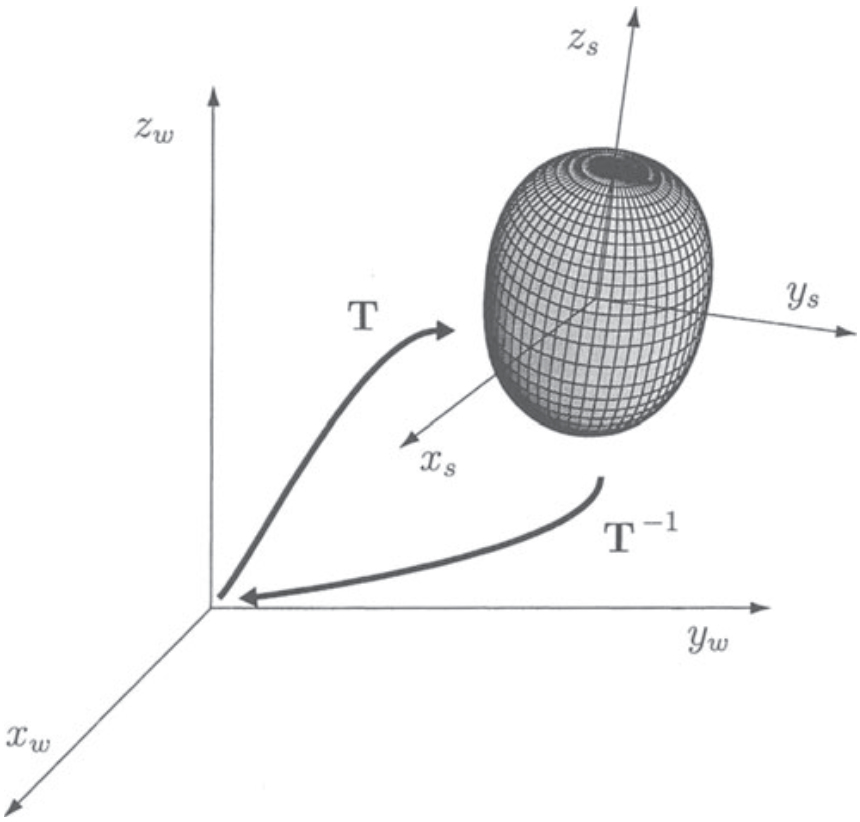
\includegraphics[width=0.35\textheight]{import/SQ_transrot}
	\caption{A SQ that has been translated and rotated by a transformation \textbf{T}. \textbf{Source}: [\citeauthor{Jaklic2000}].}
	\label{fig:SQ_transrot}
\end{figure}

\subsubsection*{Deformable Superquadrics}
\label{subsubsec:SQDeform}

Beyond simply translating and rotating a \gls{SQ}, it is also possible to deform them. It was shown in in [\citeauthor{Jaklic2000}] that \gls{SQ} can be \textit{tapered}, \textit{bent} and \textit{twisted}. 

\textbf{Tapering} involves the gradually thininng or expansion of an object along a chosen dimension. It is defined as a deformation as a function of $z$,
\begin{align}
x_D&= f_x(z)\,x_U \\
y_D&= f_y(z)\,y_U \\
z_D&= z_U,
\end{align}
where $x_U,y_U,z_U$ are components of an original undeformed surface vector $\textbf{x}_U$ and $x_D, y_D, z_D$ the components of a surface vector $\textbf{x}_D$ belonging to the deformed \gls{SQ}. The tapering functions $f_x, f_y$ work in the $x_S$-axis and $y_S$-axis directions of the \gls{SQ} centered coordinate system. In other words, the functions (linearly) offset points in the $x_S$ and $y_S$ directions respectively along the surface as a function of $z$ (along $z_S$). 

\begin{figure}[h]
	\centering
	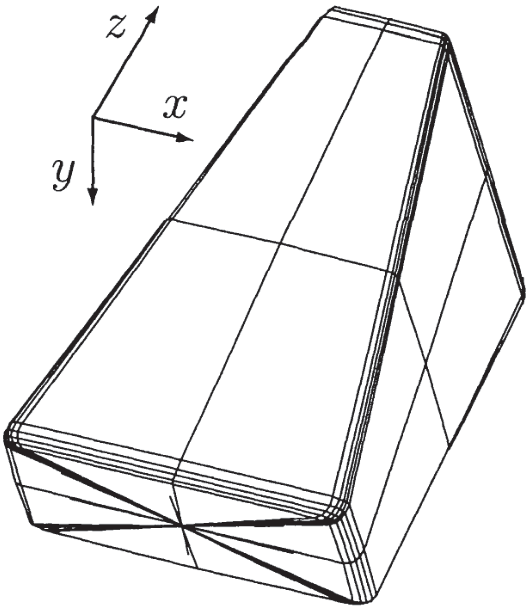
\includegraphics[width=0.15\textheight]{import/SQ_tapered}
	\caption{Tapered SQ along two axes. \textbf{Source}: [\citeauthor{Jaklic2000}].}
	\label{fig:SQ_tapered}
\end{figure}


For linear tapering, the two tapering functions are defined as,
\begin{align}
f_x(z) &= \frac{K_x}{a_3}z + 1, \hspace{0.5cm} -1 \leq K_x \\
f_y(z) &= \frac{K_y}{a_3}z + 1, \hspace{0.5cm} K_y \leq 1.
\end{align}
Thus, the two parameters $K_x$ and $K_y$ are necessary to define the (linear) tapering deformation process, corresponding to the tapering degree in each axial direction. Figure \ref{fig:SQ_tapered} shows an \gls{SQ} that has been tapered by a $f_x(z)$ and a $f_y(z)$. 

\textbf{Bending} involves transforming a straight line into a circular section, such as that of a $z_S$-axis. Note that the line segment keeps its length, which does not necessarily correspond to shape deformations when actual physical objects are bent.  The bending plane is rotated around the $z_S$-axis to an angular position defined by angle $\alpha$ (in the $x_S-y_S$-plane). The $x_U$ and $y_U$ coordinates are projected to the bending plane ($x_U,y_U \rightarrow r$), deformed (bent) using bending angle $\gamma$ in the $x_S-z_S$ or $y_S-z_S$ planes ($r \rightarrow R$), and then projected back ($R \rightarrow (x_D, y_D)$). The bending angle $\gamma$ is a function of the curvature parameter $k$ and where on the $z_S$-axis it is being evaluated.

\begin{figure}[h]
	\centering
	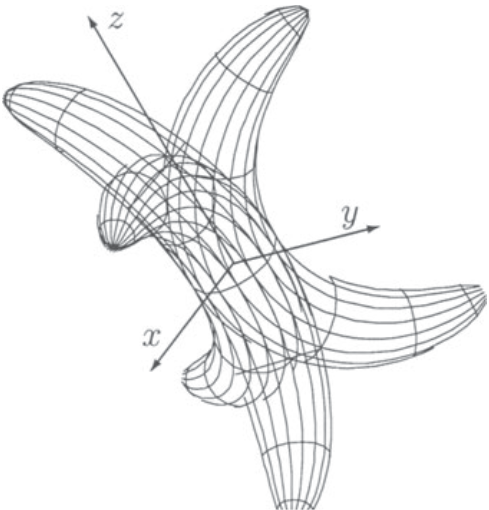
\includegraphics[width=0.25\textheight]{import/SQ_bent}
	\caption{A SQ that has been bent in three different bending planes, each of which have been rotated around the $z$-axis. \textbf{Source}: [\citeauthor{Jaklic2000}].}
	\label{fig:SQ_bent}
\end{figure}

Figure \ref{fig:SQ_bent} shows how one \gls{SQ} can look after being bent in three different planes. The transformation from bent (deformed) to unbent is given by,
\begin{align}
x_U&= x_D - (R - r)\,cos\alpha, \\
y_U&= y_D - (R - r)\,sin\alpha, \\
z_U&= \frac{1}{k}\gamma,
\end{align}
where,
\begin{equation}
\gamma = tan^{-1}\frac{z_D}{\frac{1}{k} - R},
\end{equation} 
\begin{equation}
r = \frac{1}{k} - \sqrt{z_D^2 + (\frac{1}{K} - R)^2},
\end{equation}
\begin{equation}
R = \sqrt{x_D^2 + y_D^2}cos\left(\alpha - tan^{-1} \frac{y_D}{x_D}\right).
\end{equation}
Thus, the two parameters used for doing bending are $\alpha$ and $k$. It can be interpreted that $\alpha$ is the angle around $z_S$ that decides the curving \textit{direction}, while $k$ decides \textit{how much} the \gls{SQ} will actually bend. Refer to [\citeauthor{Jaklic2000}] for details regarding the derivations of these equations.

\textbf{Twisting} is another global deformation that can be applied on a \gls{SQ}. It can be likened to twisting a deck of cards, in that the twisting happens along one axis but does not have an effect in the other axes. If the $z_S$-axis is once again used as an example, the global twist around it can be produced using the following equations [\citeauthor{Barr1984}],
\begin{align}
x_D &= x_U\,cos\xi - y_U\,sin\xi, \\
y_D &= x_U\,sin\xi + y_U\,cos\xi, \\
z_D &= z_U,
\end{align}
where crucially,
\begin{equation}
\xi = f(z_U) = f(z_D).
\end{equation}
\begin{figure}
	\centering
	\begin{minipage}[h]{0.4\textwidth}
		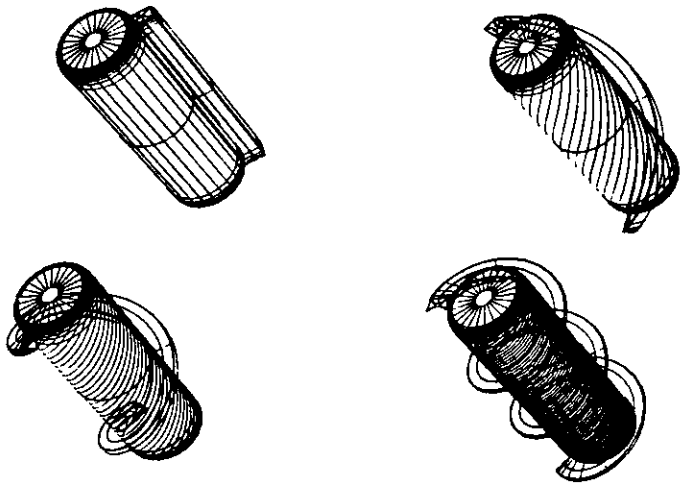
\includegraphics[width=1\textwidth]{import/SQ_twisted}
		\subcaption{The progressive twisting of two attached SQ primitives.}
		\label{fig:SQ_twist}
	\end{minipage}
	\hspace{1cm}
	\begin{minipage}[h]{0.4\textwidth}
		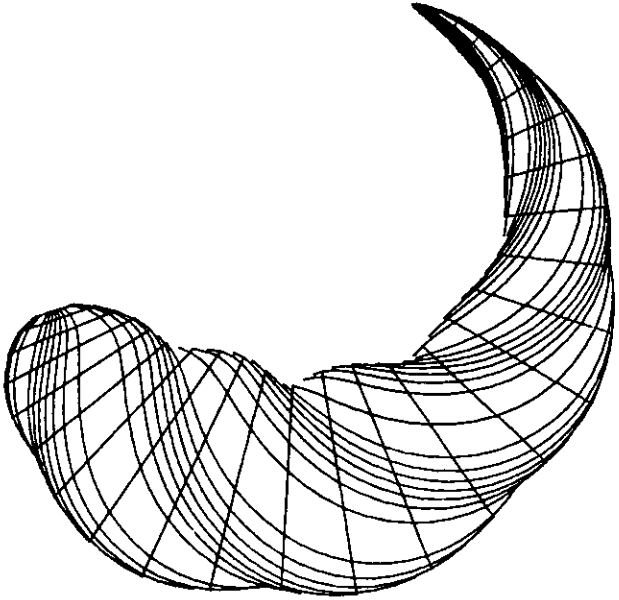
\includegraphics[width=1\textwidth]{import/SQ_bent_twisted_tapered}
		\subcaption{A bent, twisted and tapered SQ.}
		\label{fig:SQ_allDeform}
	\end{minipage}
	\caption{\textbf{Source}:[\citeauthor{Barr1984}]}
	\label{fig:SQ_combo}
\end{figure}
Figure \ref{fig:SQ_twist} clarifies the twisting deformation.

Any global deformations should be performed before performing translation and rotation. Also, note that tapering, bending and twisting (shown together in Figure \ref{fig:SQ_combo}) are not commutative operations and as such the order matters. In addition to these global deformations, it is also possible to do local deformations [\citeauthor{Jaklic2000}].


%\subsubsection{Outlier Removal}

%\subsubsection*{Distance}
%
%The true Euclidean distance between a point and a \gls{SQ} can be calculated using numerical minimization. There is no known closed form solution in the  of an algebraic expression [\citeauthor{Jaklic2000}].
%
%Skriv mer om just vad det finns för metoder?


\subsubsection{Fitting Superquadric Parameters to Range Data}

While it is perfectly possible to manually tune the $\mathbf{\Lambda}$ parameters in order to define the specific surface shape wanted, it is also possible to fit a \gls{SQ} to a cloud of points lying on the surface of an object. This can be re-framed as an optimization problem consisting of finding the \gls{SQ} that best represents an object's surface, minimizing the closest distance to each point in the point cloud.

The optimization function is as follows,
\begin{equation}
\min_{\lambda}\,\sum_{i=1}^N\left(\sqrt{\lambda_1\,\lambda_2\,\lambda_3}\left(F(x_i, y_i, z_i; \lambda_1, ..., \lambda_{11}) - 1\right)\right)^2
\label{eq:SQLoss}
\end{equation}
for \textit{N} number of points.

$\left( F( \textbf{P}, \mathbf{\Lambda}) - 1 \right)^2$ is at its minimum point when the point $\textbf{P}$	lies on the surface of the \gls{SQ} defined by $\mathbf{\Lambda}$. It features in the loss function, though the reverse is being done: finding the $\mathbf{\Lambda}$ that best fits the set of all $\textbf{P}$ points, i.e. which keeps the points as close as possible to the surface.

Due to the object self-occluding itself, it is obviously not possible to view all sides of it at the same time. The exact shape of the object can naturally not be recovered from such "degenerate" view points. Even when a "general" viewpoint is assumed, objects with surfaces where at least one principal curvature equals zero (e.g. cylinders or parallelepipeds) cannot provide sufficient constraints in order to limit the shape recovery to a unique result using only the inside-outside function by itself. The next best thing that can be done is to simply aim to reconstruct the \gls{SQ} that is the smallest. This is done by including the square root of the product of the axes scaling parameters $a_1, a_2, a_3$ (or $\lambda_1, \lambda_2, \lambda_3$), in the cost function [\citeauthor{Jaklic2000}].

Finally, it has been suggested by [\citeauthor{Jaklic2000}] that replacing $F$ with $F^{\epsilon_1}$ (or $F^{\frac{\epsilon_1}{2}}$)  would make the fitting function more suited for rapid convergence as it would make the loss function independent from the shape of the \gls{SQ} controlled by $\epsilon_1$. Compare it with Equation \ref{eq:F}. This formulation has also been present in other works ([\citeauthor{Tzovaras2007a}], [\citeauthor{Pascoal2015}]). [\citeauthor{Jaklic2000}] argue that since  $F = 1$ then $F^{\epsilon_1} = 1^{\epsilon_1}$ and the shape that is optimal will not be different. If the intention is to use the inside-outside implicit function for purposes other than as a simple "inside $F < 1$, outside $F > 1$, on surface $F = 1$" check, it will have an effect. In some works however, such as in [\citeauthor{Vezzani2018}] and its related work [\citeauthor{Fantacci2017}], the authors did not seem to use this trick.

As this is a nonlinear least squares minimization problem, the Levenberg-Marquardt method can used to solve it. Setting good initial values, if possible, is helpful to getting good performance. Also, \gls{SQ} with $\epsilon_1,\epsilon_2>2$ have concavities which make the form non-convex and can result in singularities [\citeauthor{Jaklic2000}]. Thus, inequalities limiting this should be set. Of course, it is not necessary to limit the \gls{SQ} in this way if the parameters are manually set by a human.

For the recovery of deformed \gls{SQ}, the procedure is largely the same, though the initial values should be corresponding to non-deformed \gls{SQ} (e.g., for tapering set $K_x,K_y = 0$). For bending, make sure to set $k$ to something very small but not equal to $0$, as that would result in a singularity.

%\subsubsection{Segmentation}
